\documentclass[25pt]{tikzposter}

% design based on https://twitter.com/mikemorrison/status/1110191245035479041?lang=en
% and https://github.com/SimonLarsen/tikzpostersdu

\usepackage[sfdefault]{FiraSans}
\usepackage{bm}
\usepackage{amsfonts}       % blackboard math symbols
\usepackage{amsmath}

\geometry{paperwidth=90cm, paperheight=122cm}

% metropolis colors
\definecolor{mDarkTeal}{HTML}{23373b}
\definecolor{mDarkBrown}{HTML}{604c38}
\definecolor{mLightBrown}{HTML}{EB811B}
\definecolor{mLightGreen}{HTML}{14B03D}

\usepackage{tikzposterSDU}
\usetheme{SDU}

% background color
\colorlet{blockbodybgcolor}{white}
\colorlet{backgroundcolor}{mDarkTeal}

% custom commands
\newcommand{\half}{\frac{1}{2}}
\newcommand{\x}{\bm{x}}
\newcommand{\xh}{\hat{\bm{x}}}
\newcommand{\e}{\bm{e}}
\newcommand{\z}{\bm{z}}
\newcommand{\mz}{\bm{\mu}_{z}}
\newcommand{\w}{\bm{w}}
\newcommand{\bo}{\bm{b}}
\newcommand{\A}{\bm{A}}

\newcommand{\se}{\sigma_e}
\newcommand{\sz}{\bm{\sigma_z}}
\newcommand{\laz}{\bm{\lambda}_z}

\newcommand{\X}{\bm{X}}
\newcommand{\Z}{\bm{Z}}
\newcommand{\N}{\mathcal{N}}
\newcommand{\U}{\mathcal{U}}
\newcommand{\E}[2]{\text{E}_{#1}\left[#2\right]}
\newcommand{\KL}{\text{KL}}


\begin{document}

% remove offset that would otherwise be fixed by \maketitle
\makeatletter
    \setlength{\TP@blocktop}{.47\textheight}
\makeatother

%% MAIN MESSAGE OF PAPER %%
\colorlet{blockbodybgcolor}{mDarkTeal}
\block{}{
  \color{white}{
    \fontseries{l}\fontsize{125}{150}\selectfont
    Learning \textbf{physical concepts} by \\
    \textbf{relevance determination}: Identifying \\
    \textbf{manifolds} of \textbf{differential equations.} 

    % Learning \textbf{physical concepts}  purely \\\\\\
    % from data: We demonstrate how \\\\\\
    % \textbf{generative models} can learn  \\\\\\
    % \textbf{manifolds} of \textbf{differential equations.}

    % \textbf{Relevance determination} for \\\\\\ \textbf{explainability}:
    % Learning \textbf{manifolds} of \\\\\\ sparse \textbf{differential
    % equations} from \\\\\\ \textbf{partial observations}.
  }
}
\colorlet{blockbodybgcolor}{white}


\begin{columns}
  \column{0.7}
  \block{}{
    %% TITLE OF PAPER %%
    {\Huge\bf Rodent: Relevance determination in ODE \\\\}
    {\Large Niklas Heim, V\'aclav \v Sm\'idl, Tom\'a\v s Pevn\'y} \hfill
    {\Large Czech Technical University, Prague}
  }

  \block{}{
    \begin{center}
    {\huge\bf Learning differential equations}
    \end{center}
    \begin{minipage}{.28\textwidth}
      \innerblock{}{
      \begin{itemize}
        \item We want to find the simplest ODE that describes a dynamical
          system
        \item By simple we mean: minimal order of ODE and minimum number of
          non-zero parameters.
      \end{itemize}
      }
    \end{minipage}
    \hspace{.02\textwidth}
    \begin{minipage}{.28\textwidth}
      \innerblock{}{
        \begin{itemize}
        \item Discover physically meaningful equations
          that might help understand the underlying process.
        \item We can learn manifolds of generating models not only a single process
          % \item Sparsity enforcing generative model
          % \item ODE solver acts as decoder
          % \item Latent variables are physically interpretable
          % \item Capable of learning ODE manifolds
        \end{itemize}
      }
    \end{minipage}

    \begin{tikzfigure}
      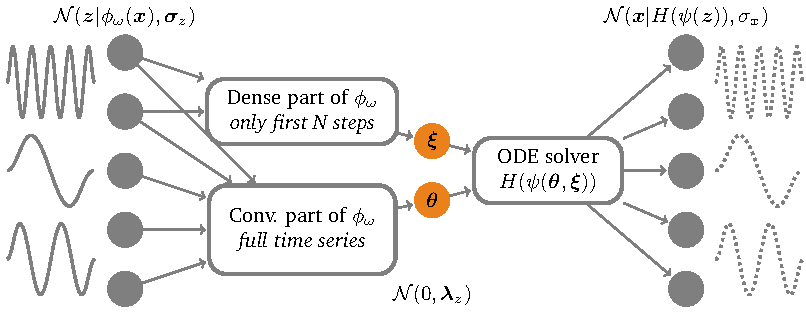
\includegraphics[width=.50\textwidth]{rodent.pdf}
    \end{tikzfigure}

    \vspace{1cm}
    \begin{center}
      {\huge\bf Manifold learning \& Reidentification}\\
    \end{center}
    \begin{tikzfigure}
      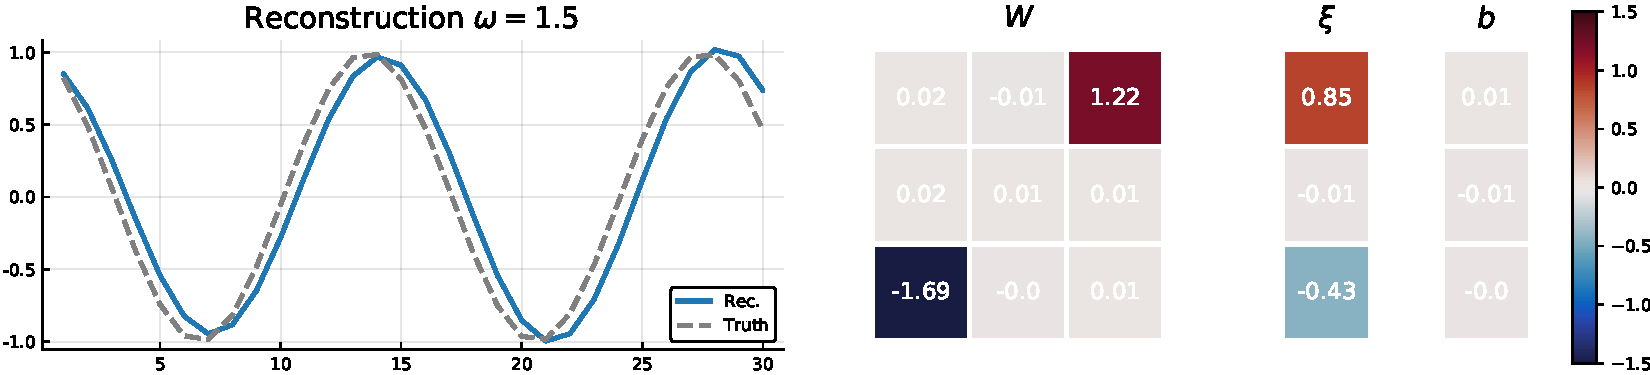
\includegraphics[width=.50\textwidth]{single_enc_rec_noreid.pdf}
    \end{tikzfigure}
    Rodent reconstructions of a harmonic signal on the left. The heatmaps on
    the right show the corresponding encodings for the weights $\bm W$, biases
    $\bm b$, and initial conditions $\bm\xi$. The Rodent reduced the latent
    space to the four truly relevant parameters.

    \begin{tikzfigure}
      \resizebox{.135\textwidth}{.11\textwidth}{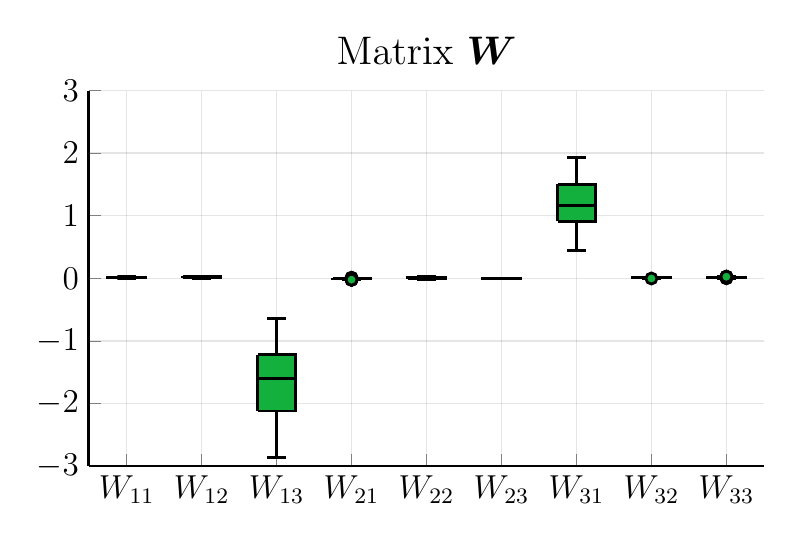
\begin{tikzpicture}[]
\begin{axis}[height = {63.50000000000001mm}, ylabel = {}, title = {Matrix $\bm W$}, xmin = {-0.0050000000000000044}, xmax = {9.005}, ymax = {3}, xlabel = {}, unbounded coords=jump,scaled x ticks = false,xlabel style = {font = {\fontsize{11 pt}{14.3 pt}\selectfont}, color = {rgb,1:red,0.00000000;green,0.00000000;blue,0.00000000}, draw opacity = 1.0, rotate = 0.0},xmajorgrids = true,xtick = {0.5,1.5,2.5,3.5,4.5,5.5,6.5,7.5,8.5},xticklabels = {$W_{11}$,$W_{12}$,$W_{13}$,$W_{21}$,$W_{22}$,$W_{23}$,$W_{31}$,$W_{32}$,$W_{33}$},xtick align = inside,xticklabel style = {font = {\fontsize{12 pt}{10.4 pt}\selectfont}, color = {rgb,1:red,0.00000000;green,0.00000000;blue,0.00000000}, draw opacity = 1.0, rotate = 0.0},x grid style = {color = {rgb,1:red,0.00000000;green,0.00000000;blue,0.00000000},
draw opacity = 0.1,
line width = 0.5,
solid},axis x line* = left,x axis line style = {color = {rgb,1:red,0.00000000;green,0.00000000;blue,0.00000000},
draw opacity = 1.0,
line width = 1,
solid},scaled y ticks = false,ylabel style = {font = {\fontsize{16 pt}{14.3 pt}\selectfont}, color = {rgb,1:red,0.00000000;green,0.00000000;blue,0.00000000}, draw opacity = 1.0, rotate = 0.0},ymajorgrids = true,ytick = {-3.0,-2.0,-1.0,0.0,1.0,2.0,3.0},yticklabels = {$-3$,$-2$,$-1$,$0$,$1$,$2$,$3$},ytick align = inside,yticklabel style = {font = {\fontsize{12 pt}{10.4 pt}\selectfont}, color = {rgb,1:red,0.00000000;green,0.00000000;blue,0.00000000}, draw opacity = 1.0, rotate = 0.0},y grid style = {color = {rgb,1:red,0.00000000;green,0.00000000;blue,0.00000000},
draw opacity = 0.1,
line width = 0.5,
solid},axis y line* = left,y axis line style = {color = {rgb,1:red,0.00000000;green,0.00000000;blue,0.00000000},
draw opacity = 1.0,
line width = 1,
solid},    xshift = 0.0mm,
    yshift = -0.0mm,
    axis background/.style={fill={rgb,1:red,1.00000000;green,1.00000000;blue,1.00000000}}
,title style = {font = {\fontsize{14 pt}{18.2 pt}\selectfont}, color = {rgb,1:red,0.00000000;green,0.00000000;blue,0.00000000}, draw opacity = 1.0, rotate = 0.0},legend style = {color = {rgb,1:red,0.00000000;green,0.00000000;blue,0.00000000},
draw opacity = 1.0,
line width = 1,
solid,fill = {rgb,1:red,1.00000000;green,1.00000000;blue,1.00000000},fill opacity = 1.0,text opacity = 1.0,font = {\fontsize{8 pt}{10.4 pt}\selectfont}},colorbar style={title=}, ymin = {-3}, width = {101.6mm}]\addplot+[draw=none, color = {rgb,1:red,0.07843137;green,0.69019608;blue,0.23921569},
draw opacity = 1.0,
line width = 0,
solid,mark = *,
mark size = 2.0,
only marks,
mark options = {
            color = {rgb,1:red,0.00000000;green,0.00000000;blue,0.00000000}, draw opacity = 1.0,
            fill = {rgb,1:red,0.07843137;green,0.69019608;blue,0.23921569}, fill opacity = 1.0,
            line width = 1,
            rotate = 0,
            solid
        },forget plot] coordinates {
(3.5, 0.003120588604360819)
(3.5, -0.022433137521147728)
(3.5, -0.02193559519946575)
(3.5, 0.010276205837726593)
(3.5, 0.0077850064262747765)
(3.5, -0.020699236541986465)
(3.5, -0.022295374423265457)
(3.5, -0.022123659029603004)
(3.5, -0.02117028273642063)
(7.5, -0.0021961559541523457)
(8.5, 0.025570224970579147)
(8.5, 0.025359224528074265)
(8.5, 0.0027110837399959564)
(8.5, 0.024966608732938766)
(8.5, 0.025552239269018173)
(8.5, 0.0019061630591750145)
(8.5, 0.023999260738492012)
(8.5, 0.02544686198234558)
};
\addplot+ [color = {rgb,1:red,0.00000000;green,0.00000000;blue,0.00000000},
draw opacity = 1.0,
line width = 1,
solid,mark = none,
mark size = 2.0,
mark options = {
            color = {rgb,1:red,0.00000000;green,0.00000000;blue,0.00000000}, draw opacity = 1.0,
            fill = {rgb,1:red,0.07843137;green,0.69019608;blue,0.23921569}, fill opacity = 1.0,
            line width = 1,
            rotate = 0,
            solid
        },fill = {rgb,1:red,0.07843137;green,0.69019608;blue,0.23921569}, fill opacity=1.0,forget plot]coordinates {
(0.5, -0.0023889392614364624)
(0.375, -0.0023889392614364624)
(0.625, -0.0023889392614364624)
(0.5, -0.0023889392614364624)
(0.5, 0.0075019001960754395)
};
\addplot+ [color = {rgb,1:red,0.00000000;green,0.00000000;blue,0.00000000},
draw opacity = 1.0,
line width = 1,
solid,mark = none,
mark size = 2.0,
mark options = {
            color = {rgb,1:red,0.00000000;green,0.00000000;blue,0.00000000}, draw opacity = 1.0,
            fill = {rgb,1:red,0.07843137;green,0.69019608;blue,0.23921569}, fill opacity = 1.0,
            line width = 1,
            rotate = 0,
            solid
        },fill = {rgb,1:red,0.07843137;green,0.69019608;blue,0.23921569}, fill opacity=1.0,forget plot]coordinates {
(0.25, 0.0075019001960754395)
(0.25, 0.015219323337078094)
(0.75, 0.015219323337078094)
(0.75, 0.0075019001960754395)
(0.25, 0.0075019001960754395)
};
\addplot+ [color = {rgb,1:red,0.00000000;green,0.00000000;blue,0.00000000},
draw opacity = 1.0,
line width = 1,
solid,mark = none,
mark size = 2.0,
mark options = {
            color = {rgb,1:red,0.00000000;green,0.00000000;blue,0.00000000}, draw opacity = 1.0,
            fill = {rgb,1:red,0.07843137;green,0.69019608;blue,0.23921569}, fill opacity = 1.0,
            line width = 1,
            rotate = 0,
            solid
        },fill = {rgb,1:red,0.07843137;green,0.69019608;blue,0.23921569}, fill opacity=1.0,forget plot]coordinates {
(0.25, 0.02049891371279955)
(0.25, 0.015219323337078094)
(0.75, 0.015219323337078094)
(0.75, 0.02049891371279955)
(0.25, 0.02049891371279955)
};
\addplot+ [color = {rgb,1:red,0.00000000;green,0.00000000;blue,0.00000000},
draw opacity = 1.0,
line width = 1,
solid,mark = none,
mark size = 2.0,
mark options = {
            color = {rgb,1:red,0.00000000;green,0.00000000;blue,0.00000000}, draw opacity = 1.0,
            fill = {rgb,1:red,0.07843137;green,0.69019608;blue,0.23921569}, fill opacity = 1.0,
            line width = 1,
            rotate = 0,
            solid
        },fill = {rgb,1:red,0.07843137;green,0.69019608;blue,0.23921569}, fill opacity=1.0,forget plot]coordinates {
(0.5, 0.03331023454666138)
(0.375, 0.03331023454666138)
(0.625, 0.03331023454666138)
(0.5, 0.03331023454666138)
(0.5, 0.02049891371279955)
};
\addplot+ [color = {rgb,1:red,0.00000000;green,0.00000000;blue,0.00000000},
draw opacity = 1.0,
line width = 1,
solid,mark = none,
mark size = 2.0,
mark options = {
            color = {rgb,1:red,0.00000000;green,0.00000000;blue,0.00000000}, draw opacity = 1.0,
            fill = {rgb,1:red,0.07843137;green,0.69019608;blue,0.23921569}, fill opacity = 1.0,
            line width = 1,
            rotate = 0,
            solid
        },fill = {rgb,1:red,0.07843137;green,0.69019608;blue,0.23921569}, fill opacity=1.0,forget plot]coordinates {
(1.5, -0.007508974522352219)
(1.375, -0.007508974522352219)
(1.625, -0.007508974522352219)
(1.5, -0.007508974522352219)
(1.5, 0.010080914478749037)
};
\addplot+ [color = {rgb,1:red,0.00000000;green,0.00000000;blue,0.00000000},
draw opacity = 1.0,
line width = 1,
solid,mark = none,
mark size = 2.0,
mark options = {
            color = {rgb,1:red,0.00000000;green,0.00000000;blue,0.00000000}, draw opacity = 1.0,
            fill = {rgb,1:red,0.07843137;green,0.69019608;blue,0.23921569}, fill opacity = 1.0,
            line width = 1,
            rotate = 0,
            solid
        },fill = {rgb,1:red,0.07843137;green,0.69019608;blue,0.23921569}, fill opacity=1.0,forget plot]coordinates {
(1.25, 0.010080914478749037)
(1.25, 0.019740505144000053)
(1.75, 0.019740505144000053)
(1.75, 0.010080914478749037)
(1.25, 0.010080914478749037)
};
\addplot+ [color = {rgb,1:red,0.00000000;green,0.00000000;blue,0.00000000},
draw opacity = 1.0,
line width = 1,
solid,mark = none,
mark size = 2.0,
mark options = {
            color = {rgb,1:red,0.00000000;green,0.00000000;blue,0.00000000}, draw opacity = 1.0,
            fill = {rgb,1:red,0.07843137;green,0.69019608;blue,0.23921569}, fill opacity = 1.0,
            line width = 1,
            rotate = 0,
            solid
        },fill = {rgb,1:red,0.07843137;green,0.69019608;blue,0.23921569}, fill opacity=1.0,forget plot]coordinates {
(1.25, 0.028870253823697567)
(1.25, 0.019740505144000053)
(1.75, 0.019740505144000053)
(1.75, 0.028870253823697567)
(1.25, 0.028870253823697567)
};
\addplot+ [color = {rgb,1:red,0.00000000;green,0.00000000;blue,0.00000000},
draw opacity = 1.0,
line width = 1,
solid,mark = none,
mark size = 2.0,
mark options = {
            color = {rgb,1:red,0.00000000;green,0.00000000;blue,0.00000000}, draw opacity = 1.0,
            fill = {rgb,1:red,0.07843137;green,0.69019608;blue,0.23921569}, fill opacity = 1.0,
            line width = 1,
            rotate = 0,
            solid
        },fill = {rgb,1:red,0.07843137;green,0.69019608;blue,0.23921569}, fill opacity=1.0,forget plot]coordinates {
(1.5, 0.0356704518198967)
(1.375, 0.0356704518198967)
(1.625, 0.0356704518198967)
(1.5, 0.0356704518198967)
(1.5, 0.028870253823697567)
};
\addplot+ [color = {rgb,1:red,0.00000000;green,0.00000000;blue,0.00000000},
draw opacity = 1.0,
line width = 1,
solid,mark = none,
mark size = 2.0,
mark options = {
            color = {rgb,1:red,0.00000000;green,0.00000000;blue,0.00000000}, draw opacity = 1.0,
            fill = {rgb,1:red,0.07843137;green,0.69019608;blue,0.23921569}, fill opacity = 1.0,
            line width = 1,
            rotate = 0,
            solid
        },fill = {rgb,1:red,0.07843137;green,0.69019608;blue,0.23921569}, fill opacity=1.0,forget plot]coordinates {
(2.5, -2.8604564666748047)
(2.375, -2.8604564666748047)
(2.625, -2.8604564666748047)
(2.5, -2.8604564666748047)
(2.5, -2.1182129979133606)
};
\addplot+ [color = {rgb,1:red,0.00000000;green,0.00000000;blue,0.00000000},
draw opacity = 1.0,
line width = 1,
solid,mark = none,
mark size = 2.0,
mark options = {
            color = {rgb,1:red,0.00000000;green,0.00000000;blue,0.00000000}, draw opacity = 1.0,
            fill = {rgb,1:red,0.07843137;green,0.69019608;blue,0.23921569}, fill opacity = 1.0,
            line width = 1,
            rotate = 0,
            solid
        },fill = {rgb,1:red,0.07843137;green,0.69019608;blue,0.23921569}, fill opacity=1.0,forget plot]coordinates {
(2.25, -2.1182129979133606)
(2.25, -1.6019176244735718)
(2.75, -1.6019176244735718)
(2.75, -2.1182129979133606)
(2.25, -2.1182129979133606)
};
\addplot+ [color = {rgb,1:red,0.00000000;green,0.00000000;blue,0.00000000},
draw opacity = 1.0,
line width = 1,
solid,mark = none,
mark size = 2.0,
mark options = {
            color = {rgb,1:red,0.00000000;green,0.00000000;blue,0.00000000}, draw opacity = 1.0,
            fill = {rgb,1:red,0.07843137;green,0.69019608;blue,0.23921569}, fill opacity = 1.0,
            line width = 1,
            rotate = 0,
            solid
        },fill = {rgb,1:red,0.07843137;green,0.69019608;blue,0.23921569}, fill opacity=1.0,forget plot]coordinates {
(2.25, -1.22038334608078)
(2.25, -1.6019176244735718)
(2.75, -1.6019176244735718)
(2.75, -1.22038334608078)
(2.25, -1.22038334608078)
};
\addplot+ [color = {rgb,1:red,0.00000000;green,0.00000000;blue,0.00000000},
draw opacity = 1.0,
line width = 1,
solid,mark = none,
mark size = 2.0,
mark options = {
            color = {rgb,1:red,0.00000000;green,0.00000000;blue,0.00000000}, draw opacity = 1.0,
            fill = {rgb,1:red,0.07843137;green,0.69019608;blue,0.23921569}, fill opacity = 1.0,
            line width = 1,
            rotate = 0,
            solid
        },fill = {rgb,1:red,0.07843137;green,0.69019608;blue,0.23921569}, fill opacity=1.0,forget plot]coordinates {
(2.5, -0.6371055841445923)
(2.375, -0.6371055841445923)
(2.625, -0.6371055841445923)
(2.5, -0.6371055841445923)
(2.5, -1.22038334608078)
};
\addplot+ [color = {rgb,1:red,0.00000000;green,0.00000000;blue,0.00000000},
draw opacity = 1.0,
line width = 1,
solid,mark = none,
mark size = 2.0,
mark options = {
            color = {rgb,1:red,0.00000000;green,0.00000000;blue,0.00000000}, draw opacity = 1.0,
            fill = {rgb,1:red,0.07843137;green,0.69019608;blue,0.23921569}, fill opacity = 1.0,
            line width = 1,
            rotate = 0,
            solid
        },fill = {rgb,1:red,0.07843137;green,0.69019608;blue,0.23921569}, fill opacity=1.0,forget plot]coordinates {
(3.5, -0.01950651779770851)
(3.375, -0.01950651779770851)
(3.625, -0.01950651779770851)
(3.5, -0.01950651779770851)
(3.5, -0.011891096131876111)
};
\addplot+ [color = {rgb,1:red,0.00000000;green,0.00000000;blue,0.00000000},
draw opacity = 1.0,
line width = 1,
solid,mark = none,
mark size = 2.0,
mark options = {
            color = {rgb,1:red,0.00000000;green,0.00000000;blue,0.00000000}, draw opacity = 1.0,
            fill = {rgb,1:red,0.07843137;green,0.69019608;blue,0.23921569}, fill opacity = 1.0,
            line width = 1,
            rotate = 0,
            solid
        },fill = {rgb,1:red,0.07843137;green,0.69019608;blue,0.23921569}, fill opacity=1.0,forget plot]coordinates {
(3.25, -0.011891096131876111)
(3.25, -0.00906949583441019)
(3.75, -0.00906949583441019)
(3.75, -0.011891096131876111)
(3.25, -0.011891096131876111)
};
\addplot+ [color = {rgb,1:red,0.00000000;green,0.00000000;blue,0.00000000},
draw opacity = 1.0,
line width = 1,
solid,mark = none,
mark size = 2.0,
mark options = {
            color = {rgb,1:red,0.00000000;green,0.00000000;blue,0.00000000}, draw opacity = 1.0,
            fill = {rgb,1:red,0.07843137;green,0.69019608;blue,0.23921569}, fill opacity = 1.0,
            line width = 1,
            rotate = 0,
            solid
        },fill = {rgb,1:red,0.07843137;green,0.69019608;blue,0.23921569}, fill opacity=1.0,forget plot]coordinates {
(3.25, -0.006252244929783046)
(3.25, -0.00906949583441019)
(3.75, -0.00906949583441019)
(3.75, -0.006252244929783046)
(3.25, -0.006252244929783046)
};
\addplot+ [color = {rgb,1:red,0.00000000;green,0.00000000;blue,0.00000000},
draw opacity = 1.0,
line width = 1,
solid,mark = none,
mark size = 2.0,
mark options = {
            color = {rgb,1:red,0.00000000;green,0.00000000;blue,0.00000000}, draw opacity = 1.0,
            fill = {rgb,1:red,0.07843137;green,0.69019608;blue,0.23921569}, fill opacity = 1.0,
            line width = 1,
            rotate = 0,
            solid
        },fill = {rgb,1:red,0.07843137;green,0.69019608;blue,0.23921569}, fill opacity=1.0,forget plot]coordinates {
(3.5, 0.000878523220308125)
(3.375, 0.000878523220308125)
(3.625, 0.000878523220308125)
(3.5, 0.000878523220308125)
(3.5, -0.006252244929783046)
};
\addplot+ [color = {rgb,1:red,0.00000000;green,0.00000000;blue,0.00000000},
draw opacity = 1.0,
line width = 1,
solid,mark = none,
mark size = 2.0,
mark options = {
            color = {rgb,1:red,0.00000000;green,0.00000000;blue,0.00000000}, draw opacity = 1.0,
            fill = {rgb,1:red,0.07843137;green,0.69019608;blue,0.23921569}, fill opacity = 1.0,
            line width = 1,
            rotate = 0,
            solid
        },fill = {rgb,1:red,0.07843137;green,0.69019608;blue,0.23921569}, fill opacity=1.0,forget plot]coordinates {
(4.5, -0.01519966870546341)
(4.375, -0.01519966870546341)
(4.625, -0.01519966870546341)
(4.5, -0.01519966870546341)
(4.5, 0.0012450776994228363)
};
\addplot+ [color = {rgb,1:red,0.00000000;green,0.00000000;blue,0.00000000},
draw opacity = 1.0,
line width = 1,
solid,mark = none,
mark size = 2.0,
mark options = {
            color = {rgb,1:red,0.00000000;green,0.00000000;blue,0.00000000}, draw opacity = 1.0,
            fill = {rgb,1:red,0.07843137;green,0.69019608;blue,0.23921569}, fill opacity = 1.0,
            line width = 1,
            rotate = 0,
            solid
        },fill = {rgb,1:red,0.07843137;green,0.69019608;blue,0.23921569}, fill opacity=1.0,forget plot]coordinates {
(4.25, 0.0012450776994228363)
(4.25, 0.010512638837099075)
(4.75, 0.010512638837099075)
(4.75, 0.0012450776994228363)
(4.25, 0.0012450776994228363)
};
\addplot+ [color = {rgb,1:red,0.00000000;green,0.00000000;blue,0.00000000},
draw opacity = 1.0,
line width = 1,
solid,mark = none,
mark size = 2.0,
mark options = {
            color = {rgb,1:red,0.00000000;green,0.00000000;blue,0.00000000}, draw opacity = 1.0,
            fill = {rgb,1:red,0.07843137;green,0.69019608;blue,0.23921569}, fill opacity = 1.0,
            line width = 1,
            rotate = 0,
            solid
        },fill = {rgb,1:red,0.07843137;green,0.69019608;blue,0.23921569}, fill opacity=1.0,forget plot]coordinates {
(4.25, 0.02138739638030529)
(4.25, 0.010512638837099075)
(4.75, 0.010512638837099075)
(4.75, 0.02138739638030529)
(4.25, 0.02138739638030529)
};
\addplot+ [color = {rgb,1:red,0.00000000;green,0.00000000;blue,0.00000000},
draw opacity = 1.0,
line width = 1,
solid,mark = none,
mark size = 2.0,
mark options = {
            color = {rgb,1:red,0.00000000;green,0.00000000;blue,0.00000000}, draw opacity = 1.0,
            fill = {rgb,1:red,0.07843137;green,0.69019608;blue,0.23921569}, fill opacity = 1.0,
            line width = 1,
            rotate = 0,
            solid
        },fill = {rgb,1:red,0.07843137;green,0.69019608;blue,0.23921569}, fill opacity=1.0,forget plot]coordinates {
(4.5, 0.03161914274096489)
(4.375, 0.03161914274096489)
(4.625, 0.03161914274096489)
(4.5, 0.03161914274096489)
(4.5, 0.02138739638030529)
};
\addplot+ [color = {rgb,1:red,0.00000000;green,0.00000000;blue,0.00000000},
draw opacity = 1.0,
line width = 1,
solid,mark = none,
mark size = 2.0,
mark options = {
            color = {rgb,1:red,0.00000000;green,0.00000000;blue,0.00000000}, draw opacity = 1.0,
            fill = {rgb,1:red,0.07843137;green,0.69019608;blue,0.23921569}, fill opacity = 1.0,
            line width = 1,
            rotate = 0,
            solid
        },fill = {rgb,1:red,0.07843137;green,0.69019608;blue,0.23921569}, fill opacity=1.0,forget plot]coordinates {
(5.5, -0.00833897478878498)
(5.375, -0.00833897478878498)
(5.625, -0.00833897478878498)
(5.5, -0.00833897478878498)
(5.5, -0.004387741908431053)
};
\addplot+ [color = {rgb,1:red,0.00000000;green,0.00000000;blue,0.00000000},
draw opacity = 1.0,
line width = 1,
solid,mark = none,
mark size = 2.0,
mark options = {
            color = {rgb,1:red,0.00000000;green,0.00000000;blue,0.00000000}, draw opacity = 1.0,
            fill = {rgb,1:red,0.07843137;green,0.69019608;blue,0.23921569}, fill opacity = 1.0,
            line width = 1,
            rotate = 0,
            solid
        },fill = {rgb,1:red,0.07843137;green,0.69019608;blue,0.23921569}, fill opacity=1.0,forget plot]coordinates {
(5.25, -0.004387741908431053)
(5.25, -0.0017924816347658634)
(5.75, -0.0017924816347658634)
(5.75, -0.004387741908431053)
(5.25, -0.004387741908431053)
};
\addplot+ [color = {rgb,1:red,0.00000000;green,0.00000000;blue,0.00000000},
draw opacity = 1.0,
line width = 1,
solid,mark = none,
mark size = 2.0,
mark options = {
            color = {rgb,1:red,0.00000000;green,0.00000000;blue,0.00000000}, draw opacity = 1.0,
            fill = {rgb,1:red,0.07843137;green,0.69019608;blue,0.23921569}, fill opacity = 1.0,
            line width = 1,
            rotate = 0,
            solid
        },fill = {rgb,1:red,0.07843137;green,0.69019608;blue,0.23921569}, fill opacity=1.0,forget plot]coordinates {
(5.25, -0.0002617044374346733)
(5.25, -0.0017924816347658634)
(5.75, -0.0017924816347658634)
(5.75, -0.0002617044374346733)
(5.25, -0.0002617044374346733)
};
\addplot+ [color = {rgb,1:red,0.00000000;green,0.00000000;blue,0.00000000},
draw opacity = 1.0,
line width = 1,
solid,mark = none,
mark size = 2.0,
mark options = {
            color = {rgb,1:red,0.00000000;green,0.00000000;blue,0.00000000}, draw opacity = 1.0,
            fill = {rgb,1:red,0.07843137;green,0.69019608;blue,0.23921569}, fill opacity = 1.0,
            line width = 1,
            rotate = 0,
            solid
        },fill = {rgb,1:red,0.07843137;green,0.69019608;blue,0.23921569}, fill opacity=1.0,forget plot]coordinates {
(5.5, 0.002932983450591564)
(5.375, 0.002932983450591564)
(5.625, 0.002932983450591564)
(5.5, 0.002932983450591564)
(5.5, -0.0002617044374346733)
};
\addplot+ [color = {rgb,1:red,0.00000000;green,0.00000000;blue,0.00000000},
draw opacity = 1.0,
line width = 1,
solid,mark = none,
mark size = 2.0,
mark options = {
            color = {rgb,1:red,0.00000000;green,0.00000000;blue,0.00000000}, draw opacity = 1.0,
            fill = {rgb,1:red,0.07843137;green,0.69019608;blue,0.23921569}, fill opacity = 1.0,
            line width = 1,
            rotate = 0,
            solid
        },fill = {rgb,1:red,0.07843137;green,0.69019608;blue,0.23921569}, fill opacity=1.0,forget plot]coordinates {
(6.5, 0.4462711811065674)
(6.375, 0.4462711811065674)
(6.625, 0.4462711811065674)
(6.5, 0.4462711811065674)
(6.5, 0.9143857657909393)
};
\addplot+ [color = {rgb,1:red,0.00000000;green,0.00000000;blue,0.00000000},
draw opacity = 1.0,
line width = 1,
solid,mark = none,
mark size = 2.0,
mark options = {
            color = {rgb,1:red,0.00000000;green,0.00000000;blue,0.00000000}, draw opacity = 1.0,
            fill = {rgb,1:red,0.07843137;green,0.69019608;blue,0.23921569}, fill opacity = 1.0,
            line width = 1,
            rotate = 0,
            solid
        },fill = {rgb,1:red,0.07843137;green,0.69019608;blue,0.23921569}, fill opacity=1.0,forget plot]coordinates {
(6.25, 0.9143857657909393)
(6.25, 1.16566002368927)
(6.75, 1.16566002368927)
(6.75, 0.9143857657909393)
(6.25, 0.9143857657909393)
};
\addplot+ [color = {rgb,1:red,0.00000000;green,0.00000000;blue,0.00000000},
draw opacity = 1.0,
line width = 1,
solid,mark = none,
mark size = 2.0,
mark options = {
            color = {rgb,1:red,0.00000000;green,0.00000000;blue,0.00000000}, draw opacity = 1.0,
            fill = {rgb,1:red,0.07843137;green,0.69019608;blue,0.23921569}, fill opacity = 1.0,
            line width = 1,
            rotate = 0,
            solid
        },fill = {rgb,1:red,0.07843137;green,0.69019608;blue,0.23921569}, fill opacity=1.0,forget plot]coordinates {
(6.25, 1.5006077289581299)
(6.25, 1.16566002368927)
(6.75, 1.16566002368927)
(6.75, 1.5006077289581299)
(6.25, 1.5006077289581299)
};
\addplot+ [color = {rgb,1:red,0.00000000;green,0.00000000;blue,0.00000000},
draw opacity = 1.0,
line width = 1,
solid,mark = none,
mark size = 2.0,
mark options = {
            color = {rgb,1:red,0.00000000;green,0.00000000;blue,0.00000000}, draw opacity = 1.0,
            fill = {rgb,1:red,0.07843137;green,0.69019608;blue,0.23921569}, fill opacity = 1.0,
            line width = 1,
            rotate = 0,
            solid
        },fill = {rgb,1:red,0.07843137;green,0.69019608;blue,0.23921569}, fill opacity=1.0,forget plot]coordinates {
(6.5, 1.9340778589248657)
(6.375, 1.9340778589248657)
(6.625, 1.9340778589248657)
(6.5, 1.9340778589248657)
(6.5, 1.5006077289581299)
};
\addplot+ [color = {rgb,1:red,0.00000000;green,0.00000000;blue,0.00000000},
draw opacity = 1.0,
line width = 1,
solid,mark = none,
mark size = 2.0,
mark options = {
            color = {rgb,1:red,0.00000000;green,0.00000000;blue,0.00000000}, draw opacity = 1.0,
            fill = {rgb,1:red,0.07843137;green,0.69019608;blue,0.23921569}, fill opacity = 1.0,
            line width = 1,
            rotate = 0,
            solid
        },fill = {rgb,1:red,0.07843137;green,0.69019608;blue,0.23921569}, fill opacity=1.0,forget plot]coordinates {
(7.5, -0.0002535148523747921)
(7.375, -0.0002535148523747921)
(7.625, -0.0002535148523747921)
(7.5, -0.0002535148523747921)
(7.5, 0.007277090917341411)
};
\addplot+ [color = {rgb,1:red,0.00000000;green,0.00000000;blue,0.00000000},
draw opacity = 1.0,
line width = 1,
solid,mark = none,
mark size = 2.0,
mark options = {
            color = {rgb,1:red,0.00000000;green,0.00000000;blue,0.00000000}, draw opacity = 1.0,
            fill = {rgb,1:red,0.07843137;green,0.69019608;blue,0.23921569}, fill opacity = 1.0,
            line width = 1,
            rotate = 0,
            solid
        },fill = {rgb,1:red,0.07843137;green,0.69019608;blue,0.23921569}, fill opacity=1.0,forget plot]coordinates {
(7.25, 0.007277090917341411)
(7.25, 0.009713097475469112)
(7.75, 0.009713097475469112)
(7.75, 0.007277090917341411)
(7.25, 0.007277090917341411)
};
\addplot+ [color = {rgb,1:red,0.00000000;green,0.00000000;blue,0.00000000},
draw opacity = 1.0,
line width = 1,
solid,mark = none,
mark size = 2.0,
mark options = {
            color = {rgb,1:red,0.00000000;green,0.00000000;blue,0.00000000}, draw opacity = 1.0,
            fill = {rgb,1:red,0.07843137;green,0.69019608;blue,0.23921569}, fill opacity = 1.0,
            line width = 1,
            rotate = 0,
            solid
        },fill = {rgb,1:red,0.07843137;green,0.69019608;blue,0.23921569}, fill opacity=1.0,forget plot]coordinates {
(7.25, 0.013498167973011732)
(7.25, 0.009713097475469112)
(7.75, 0.009713097475469112)
(7.75, 0.013498167973011732)
(7.25, 0.013498167973011732)
};
\addplot+ [color = {rgb,1:red,0.00000000;green,0.00000000;blue,0.00000000},
draw opacity = 1.0,
line width = 1,
solid,mark = none,
mark size = 2.0,
mark options = {
            color = {rgb,1:red,0.00000000;green,0.00000000;blue,0.00000000}, draw opacity = 1.0,
            fill = {rgb,1:red,0.07843137;green,0.69019608;blue,0.23921569}, fill opacity = 1.0,
            line width = 1,
            rotate = 0,
            solid
        },fill = {rgb,1:red,0.07843137;green,0.69019608;blue,0.23921569}, fill opacity=1.0,forget plot]coordinates {
(7.5, 0.020075445994734764)
(7.375, 0.020075445994734764)
(7.625, 0.020075445994734764)
(7.5, 0.020075445994734764)
(7.5, 0.013498167973011732)
};
\addplot+ [color = {rgb,1:red,0.00000000;green,0.00000000;blue,0.00000000},
draw opacity = 1.0,
line width = 1,
solid,mark = none,
mark size = 2.0,
mark options = {
            color = {rgb,1:red,0.00000000;green,0.00000000;blue,0.00000000}, draw opacity = 1.0,
            fill = {rgb,1:red,0.07843137;green,0.69019608;blue,0.23921569}, fill opacity = 1.0,
            line width = 1,
            rotate = 0,
            solid
        },fill = {rgb,1:red,0.07843137;green,0.69019608;blue,0.23921569}, fill opacity=1.0,forget plot]coordinates {
(8.5, 0.0035375477746129036)
(8.375, 0.0035375477746129036)
(8.625, 0.0035375477746129036)
(8.5, 0.0035375477746129036)
(8.5, 0.010756546165794134)
};
\addplot+ [color = {rgb,1:red,0.00000000;green,0.00000000;blue,0.00000000},
draw opacity = 1.0,
line width = 1,
solid,mark = none,
mark size = 2.0,
mark options = {
            color = {rgb,1:red,0.00000000;green,0.00000000;blue,0.00000000}, draw opacity = 1.0,
            fill = {rgb,1:red,0.07843137;green,0.69019608;blue,0.23921569}, fill opacity = 1.0,
            line width = 1,
            rotate = 0,
            solid
        },fill = {rgb,1:red,0.07843137;green,0.69019608;blue,0.23921569}, fill opacity=1.0,forget plot]coordinates {
(8.25, 0.010756546165794134)
(8.25, 0.012593354098498821)
(8.75, 0.012593354098498821)
(8.75, 0.010756546165794134)
(8.25, 0.010756546165794134)
};
\addplot+ [color = {rgb,1:red,0.00000000;green,0.00000000;blue,0.00000000},
draw opacity = 1.0,
line width = 1,
solid,mark = none,
mark size = 2.0,
mark options = {
            color = {rgb,1:red,0.00000000;green,0.00000000;blue,0.00000000}, draw opacity = 1.0,
            fill = {rgb,1:red,0.07843137;green,0.69019608;blue,0.23921569}, fill opacity = 1.0,
            line width = 1,
            rotate = 0,
            solid
        },fill = {rgb,1:red,0.07843137;green,0.69019608;blue,0.23921569}, fill opacity=1.0,forget plot]coordinates {
(8.25, 0.01595639670267701)
(8.25, 0.012593354098498821)
(8.75, 0.012593354098498821)
(8.75, 0.01595639670267701)
(8.25, 0.01595639670267701)
};
\addplot+ [color = {rgb,1:red,0.00000000;green,0.00000000;blue,0.00000000},
draw opacity = 1.0,
line width = 1,
solid,mark = none,
mark size = 2.0,
mark options = {
            color = {rgb,1:red,0.00000000;green,0.00000000;blue,0.00000000}, draw opacity = 1.0,
            fill = {rgb,1:red,0.07843137;green,0.69019608;blue,0.23921569}, fill opacity = 1.0,
            line width = 1,
            rotate = 0,
            solid
        },fill = {rgb,1:red,0.07843137;green,0.69019608;blue,0.23921569}, fill opacity=1.0,forget plot]coordinates {
(8.5, 0.023572349920868874)
(8.375, 0.023572349920868874)
(8.625, 0.023572349920868874)
(8.5, 0.023572349920868874)
(8.5, 0.01595639670267701)
};
\end{axis}

\end{tikzpicture}
}
      \resizebox{.075\textwidth}{.11\textwidth}{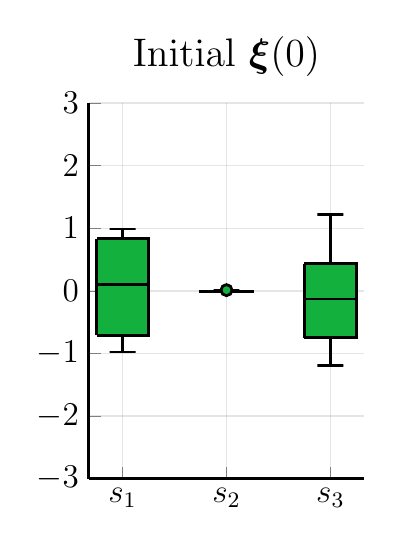
\begin{tikzpicture}[]
\begin{axis}[height = {63.50000000000001mm}, ylabel = {}, title = {Initial $\bm \xi(0)$}, xmin = {0.175}, xmax = {2.825}, ymax = {3}, xlabel = {}, unbounded coords=jump,scaled x ticks = false,xlabel style = {font = {\fontsize{16 pt}{14.3 pt}\selectfont}, color = {rgb,1:red,0.00000000;green,0.00000000;blue,0.00000000}, draw opacity = 1.0, rotate = 0.0},xmajorgrids = true,xtick = {0.5,1.5,2.5},xticklabels = {$s_1$,$s_2$,$s_3$},xtick align = inside,xticklabel style = {font = {\fontsize{12 pt}{10.4 pt}\selectfont}, color = {rgb,1:red,0.00000000;green,0.00000000;blue,0.00000000}, draw opacity = 1.0, rotate = 0.0},x grid style = {color = {rgb,1:red,0.00000000;green,0.00000000;blue,0.00000000},
draw opacity = 0.1,
line width = 0.5,
solid},axis x line* = left,x axis line style = {color = {rgb,1:red,0.00000000;green,0.00000000;blue,0.00000000},
draw opacity = 1.0,
line width = 1,
solid},scaled y ticks = false,ylabel style = {font = {\fontsize{16 pt}{14.3 pt}\selectfont}, color = {rgb,1:red,0.00000000;green,0.00000000;blue,0.00000000}, draw opacity = 1.0, rotate = 0.0},ymajorgrids = true,ytick = {-3.0,-2.0,-1.0,0.0,1.0,2.0,3.0},yticklabels = {$-3$,$-2$,$-1$,$0$,$1$,$2$,$3$},ytick align = inside,yticklabel style = {font = {\fontsize{12 pt}{10.4 pt}\selectfont}, color = {rgb,1:red,0.00000000;green,0.00000000;blue,0.00000000}, draw opacity = 1.0, rotate = 0.0},y grid style = {color = {rgb,1:red,0.00000000;green,0.00000000;blue,0.00000000},
draw opacity = 0.1,
line width = 0.5,
solid},axis y line* = left,y axis line style = {color = {rgb,1:red,0.00000000;green,0.00000000;blue,0.00000000},
draw opacity = 1.0,
line width = 1,
solid},    xshift = 0.0mm,
    yshift = -0.0mm,
    axis background/.style={fill={rgb,1:red,1.00000000;green,1.00000000;blue,1.00000000}}
,title style = {font = {\fontsize{14 pt}{18.2 pt}\selectfont}, color = {rgb,1:red,0.00000000;green,0.00000000;blue,0.00000000}, draw opacity = 1.0, rotate = 0.0},legend style = {color = {rgb,1:red,0.00000000;green,0.00000000;blue,0.00000000},
draw opacity = 1.0,
line width = 1,
solid,fill = {rgb,1:red,1.00000000;green,1.00000000;blue,1.00000000},fill opacity = 1.0,text opacity = 1.0,font = {\fontsize{8 pt}{10.4 pt}\selectfont}},colorbar style={title=}, ymin = {-3}, width = {50.8mm}]\addplot+[draw=none, color = {rgb,1:red,0.07843137;green,0.69019608;blue,0.23921569},
draw opacity = 1.0,
line width = 0,
solid,mark = *,
mark size = 2.0,
only marks,
mark options = {
            color = {rgb,1:red,0.00000000;green,0.00000000;blue,0.00000000}, draw opacity = 1.0,
            fill = {rgb,1:red,0.07843137;green,0.69019608;blue,0.23921569}, fill opacity = 1.0,
            line width = 1,
            rotate = 0,
            solid
        },forget plot] coordinates {
(1.5, 0.011398278176784515)
};
\addplot+ [color = {rgb,1:red,0.00000000;green,0.00000000;blue,0.00000000},
draw opacity = 1.0,
line width = 1,
solid,mark = none,
mark size = 2.0,
mark options = {
            color = {rgb,1:red,0.00000000;green,0.00000000;blue,0.00000000}, draw opacity = 1.0,
            fill = {rgb,1:red,0.07843137;green,0.69019608;blue,0.23921569}, fill opacity = 1.0,
            line width = 1,
            rotate = 0,
            solid
        },fill = {rgb,1:red,0.07843137;green,0.69019608;blue,0.23921569}, fill opacity=1.0,forget plot]coordinates {
(0.5, -0.9768325686454773)
(0.375, -0.9768325686454773)
(0.625, -0.9768325686454773)
(0.5, -0.9768325686454773)
(0.5, -0.7117224782705307)
};
\addplot+ [color = {rgb,1:red,0.00000000;green,0.00000000;blue,0.00000000},
draw opacity = 1.0,
line width = 1,
solid,mark = none,
mark size = 2.0,
mark options = {
            color = {rgb,1:red,0.00000000;green,0.00000000;blue,0.00000000}, draw opacity = 1.0,
            fill = {rgb,1:red,0.07843137;green,0.69019608;blue,0.23921569}, fill opacity = 1.0,
            line width = 1,
            rotate = 0,
            solid
        },fill = {rgb,1:red,0.07843137;green,0.69019608;blue,0.23921569}, fill opacity=1.0,forget plot]coordinates {
(0.25, -0.7117224782705307)
(0.25, 0.09610114246606827)
(0.75, 0.09610114246606827)
(0.75, -0.7117224782705307)
(0.25, -0.7117224782705307)
};
\addplot+ [color = {rgb,1:red,0.00000000;green,0.00000000;blue,0.00000000},
draw opacity = 1.0,
line width = 1,
solid,mark = none,
mark size = 2.0,
mark options = {
            color = {rgb,1:red,0.00000000;green,0.00000000;blue,0.00000000}, draw opacity = 1.0,
            fill = {rgb,1:red,0.07843137;green,0.69019608;blue,0.23921569}, fill opacity = 1.0,
            line width = 1,
            rotate = 0,
            solid
        },fill = {rgb,1:red,0.07843137;green,0.69019608;blue,0.23921569}, fill opacity=1.0,forget plot]coordinates {
(0.25, 0.8310767263174057)
(0.25, 0.09610114246606827)
(0.75, 0.09610114246606827)
(0.75, 0.8310767263174057)
(0.25, 0.8310767263174057)
};
\addplot+ [color = {rgb,1:red,0.00000000;green,0.00000000;blue,0.00000000},
draw opacity = 1.0,
line width = 1,
solid,mark = none,
mark size = 2.0,
mark options = {
            color = {rgb,1:red,0.00000000;green,0.00000000;blue,0.00000000}, draw opacity = 1.0,
            fill = {rgb,1:red,0.07843137;green,0.69019608;blue,0.23921569}, fill opacity = 1.0,
            line width = 1,
            rotate = 0,
            solid
        },fill = {rgb,1:red,0.07843137;green,0.69019608;blue,0.23921569}, fill opacity=1.0,forget plot]coordinates {
(0.5, 0.9884899258613586)
(0.375, 0.9884899258613586)
(0.625, 0.9884899258613586)
(0.5, 0.9884899258613586)
(0.5, 0.8310767263174057)
};
\addplot+ [color = {rgb,1:red,0.00000000;green,0.00000000;blue,0.00000000},
draw opacity = 1.0,
line width = 1,
solid,mark = none,
mark size = 2.0,
mark options = {
            color = {rgb,1:red,0.00000000;green,0.00000000;blue,0.00000000}, draw opacity = 1.0,
            fill = {rgb,1:red,0.07843137;green,0.69019608;blue,0.23921569}, fill opacity = 1.0,
            line width = 1,
            rotate = 0,
            solid
        },fill = {rgb,1:red,0.07843137;green,0.69019608;blue,0.23921569}, fill opacity=1.0,forget plot]coordinates {
(1.5, -0.019915202632546425)
(1.375, -0.019915202632546425)
(1.625, -0.019915202632546425)
(1.5, -0.019915202632546425)
(1.5, -0.008746073115617037)
};
\addplot+ [color = {rgb,1:red,0.00000000;green,0.00000000;blue,0.00000000},
draw opacity = 1.0,
line width = 1,
solid,mark = none,
mark size = 2.0,
mark options = {
            color = {rgb,1:red,0.00000000;green,0.00000000;blue,0.00000000}, draw opacity = 1.0,
            fill = {rgb,1:red,0.07843137;green,0.69019608;blue,0.23921569}, fill opacity = 1.0,
            line width = 1,
            rotate = 0,
            solid
        },fill = {rgb,1:red,0.07843137;green,0.69019608;blue,0.23921569}, fill opacity=1.0,forget plot]coordinates {
(1.25, -0.008746073115617037)
(1.25, -0.00513463094830513)
(1.75, -0.00513463094830513)
(1.75, -0.008746073115617037)
(1.25, -0.008746073115617037)
};
\addplot+ [color = {rgb,1:red,0.00000000;green,0.00000000;blue,0.00000000},
draw opacity = 1.0,
line width = 1,
solid,mark = none,
mark size = 2.0,
mark options = {
            color = {rgb,1:red,0.00000000;green,0.00000000;blue,0.00000000}, draw opacity = 1.0,
            fill = {rgb,1:red,0.07843137;green,0.69019608;blue,0.23921569}, fill opacity = 1.0,
            line width = 1,
            rotate = 0,
            solid
        },fill = {rgb,1:red,0.07843137;green,0.69019608;blue,0.23921569}, fill opacity=1.0,forget plot]coordinates {
(1.25, -0.0008138759294524789)
(1.25, -0.00513463094830513)
(1.75, -0.00513463094830513)
(1.75, -0.0008138759294524789)
(1.25, -0.0008138759294524789)
};
\addplot+ [color = {rgb,1:red,0.00000000;green,0.00000000;blue,0.00000000},
draw opacity = 1.0,
line width = 1,
solid,mark = none,
mark size = 2.0,
mark options = {
            color = {rgb,1:red,0.00000000;green,0.00000000;blue,0.00000000}, draw opacity = 1.0,
            fill = {rgb,1:red,0.07843137;green,0.69019608;blue,0.23921569}, fill opacity = 1.0,
            line width = 1,
            rotate = 0,
            solid
        },fill = {rgb,1:red,0.07843137;green,0.69019608;blue,0.23921569}, fill opacity=1.0,forget plot]coordinates {
(1.5, 0.008533485233783722)
(1.375, 0.008533485233783722)
(1.625, 0.008533485233783722)
(1.5, 0.008533485233783722)
(1.5, -0.0008138759294524789)
};
\addplot+ [color = {rgb,1:red,0.00000000;green,0.00000000;blue,0.00000000},
draw opacity = 1.0,
line width = 1,
solid,mark = none,
mark size = 2.0,
mark options = {
            color = {rgb,1:red,0.00000000;green,0.00000000;blue,0.00000000}, draw opacity = 1.0,
            fill = {rgb,1:red,0.07843137;green,0.69019608;blue,0.23921569}, fill opacity = 1.0,
            line width = 1,
            rotate = 0,
            solid
        },fill = {rgb,1:red,0.07843137;green,0.69019608;blue,0.23921569}, fill opacity=1.0,forget plot]coordinates {
(2.5, -1.1973670721054077)
(2.375, -1.1973670721054077)
(2.625, -1.1973670721054077)
(2.5, -1.1973670721054077)
(2.5, -0.7456951588392258)
};
\addplot+ [color = {rgb,1:red,0.00000000;green,0.00000000;blue,0.00000000},
draw opacity = 1.0,
line width = 1,
solid,mark = none,
mark size = 2.0,
mark options = {
            color = {rgb,1:red,0.00000000;green,0.00000000;blue,0.00000000}, draw opacity = 1.0,
            fill = {rgb,1:red,0.07843137;green,0.69019608;blue,0.23921569}, fill opacity = 1.0,
            line width = 1,
            rotate = 0,
            solid
        },fill = {rgb,1:red,0.07843137;green,0.69019608;blue,0.23921569}, fill opacity=1.0,forget plot]coordinates {
(2.25, -0.7456951588392258)
(2.25, -0.12840958312153816)
(2.75, -0.12840958312153816)
(2.75, -0.7456951588392258)
(2.25, -0.7456951588392258)
};
\addplot+ [color = {rgb,1:red,0.00000000;green,0.00000000;blue,0.00000000},
draw opacity = 1.0,
line width = 1,
solid,mark = none,
mark size = 2.0,
mark options = {
            color = {rgb,1:red,0.00000000;green,0.00000000;blue,0.00000000}, draw opacity = 1.0,
            fill = {rgb,1:red,0.07843137;green,0.69019608;blue,0.23921569}, fill opacity = 1.0,
            line width = 1,
            rotate = 0,
            solid
        },fill = {rgb,1:red,0.07843137;green,0.69019608;blue,0.23921569}, fill opacity=1.0,forget plot]coordinates {
(2.25, 0.4327097311615944)
(2.25, -0.12840958312153816)
(2.75, -0.12840958312153816)
(2.75, 0.4327097311615944)
(2.25, 0.4327097311615944)
};
\addplot+ [color = {rgb,1:red,0.00000000;green,0.00000000;blue,0.00000000},
draw opacity = 1.0,
line width = 1,
solid,mark = none,
mark size = 2.0,
mark options = {
            color = {rgb,1:red,0.00000000;green,0.00000000;blue,0.00000000}, draw opacity = 1.0,
            fill = {rgb,1:red,0.07843137;green,0.69019608;blue,0.23921569}, fill opacity = 1.0,
            line width = 1,
            rotate = 0,
            solid
        },fill = {rgb,1:red,0.07843137;green,0.69019608;blue,0.23921569}, fill opacity=1.0,forget plot]coordinates {
(2.5, 1.2212475538253784)
(2.375, 1.2212475538253784)
(2.625, 1.2212475538253784)
(2.5, 1.2212475538253784)
(2.5, 0.4327097311615944)
};
\end{axis}

\end{tikzpicture}
}
      \resizebox{.075\textwidth}{.11\textwidth}{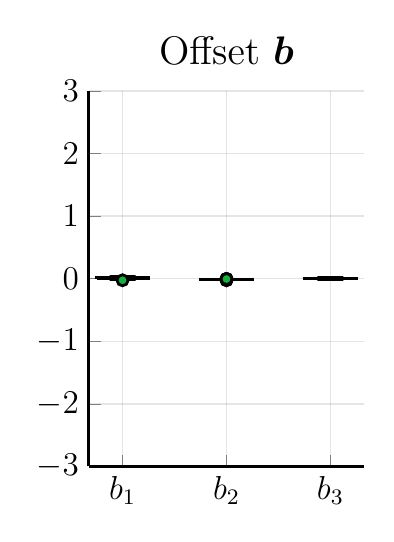
\begin{tikzpicture}[]
\begin{axis}[height = {63.50000000000001mm}, ylabel = {}, title = {Offset $\bm b$}, xmin = {0.175}, xmax = {2.825}, ymax = {3}, xlabel = {}, unbounded coords=jump,scaled x ticks = false,xlabel style = {font = {\fontsize{11 pt}{14.3 pt}\selectfont}, color = {rgb,1:red,0.00000000;green,0.00000000;blue,0.00000000}, draw opacity = 1.0, rotate = 0.0},xmajorgrids = true,xtick = {0.5,1.5,2.5},xticklabels = {$b_1$,$b_2$,$b_3$},xtick align = inside,xticklabel style = {font = {\fontsize{12 pt}{10.4 pt}\selectfont}, color = {rgb,1:red,0.00000000;green,0.00000000;blue,0.00000000}, draw opacity = 1.0, rotate = 0.0},x grid style = {color = {rgb,1:red,0.00000000;green,0.00000000;blue,0.00000000},
draw opacity = 0.1,
line width = 0.5,
solid},axis x line* = left,x axis line style = {color = {rgb,1:red,0.00000000;green,0.00000000;blue,0.00000000},
draw opacity = 1.0,
line width = 1,
solid},scaled y ticks = false,ylabel style = {font = {\fontsize{11 pt}{14.3 pt}\selectfont}, color = {rgb,1:red,0.00000000;green,0.00000000;blue,0.00000000}, draw opacity = 1.0, rotate = 0.0},ymajorgrids = true,ytick = {-3.0,-2.0,-1.0,0.0,1.0,2.0,3.0},yticklabels = {$-3$,$-2$,$-1$,$0$,$1$,$2$,$3$},ytick align = inside,yticklabel style = {font = {\fontsize{12 pt}{10.4 pt}\selectfont}, color = {rgb,1:red,0.00000000;green,0.00000000;blue,0.00000000}, draw opacity = 1.0, rotate = 0.0},y grid style = {color = {rgb,1:red,0.00000000;green,0.00000000;blue,0.00000000},
draw opacity = 0.1,
line width = 0.5,
solid},axis y line* = left,y axis line style = {color = {rgb,1:red,0.00000000;green,0.00000000;blue,0.00000000},
draw opacity = 1.0,
line width = 1,
solid},    xshift = 0.0mm,
    yshift = -0.0mm,
    axis background/.style={fill={rgb,1:red,1.00000000;green,1.00000000;blue,1.00000000}}
,title style = {font = {\fontsize{14 pt}{18.2 pt}\selectfont}, color = {rgb,1:red,0.00000000;green,0.00000000;blue,0.00000000}, draw opacity = 1.0, rotate = 0.0},legend style = {color = {rgb,1:red,0.00000000;green,0.00000000;blue,0.00000000},
draw opacity = 1.0,
line width = 1,
solid,fill = {rgb,1:red,1.00000000;green,1.00000000;blue,1.00000000},fill opacity = 1.0,text opacity = 1.0,font = {\fontsize{8 pt}{10.4 pt}\selectfont}},colorbar style={title=}, ymin = {-3}, width = {50.8mm}]\addplot+[draw=none, color = {rgb,1:red,0.07843137;green,0.69019608;blue,0.23921569},
draw opacity = 1.0,
line width = 0,
solid,mark = *,
mark size = 2.0,
only marks,
mark options = {
            color = {rgb,1:red,0.00000000;green,0.00000000;blue,0.00000000}, draw opacity = 1.0,
            fill = {rgb,1:red,0.07843137;green,0.69019608;blue,0.23921569}, fill opacity = 1.0,
            line width = 1,
            rotate = 0,
            solid
        },forget plot] coordinates {
(0.5, -0.025126254186034203)
(1.5, -0.005002434831112623)
(1.5, -0.0056295618414878845)
(1.5, -0.022652413696050644)
(1.5, -0.02546759322285652)
(1.5, -0.004970291163772345)
(1.5, -0.005505470559000969)
(1.5, -0.005920222960412502)
};
\addplot+ [color = {rgb,1:red,0.00000000;green,0.00000000;blue,0.00000000},
draw opacity = 1.0,
line width = 1,
solid,mark = none,
mark size = 2.0,
mark options = {
            color = {rgb,1:red,0.00000000;green,0.00000000;blue,0.00000000}, draw opacity = 1.0,
            fill = {rgb,1:red,0.07843137;green,0.69019608;blue,0.23921569}, fill opacity = 1.0,
            line width = 1,
            rotate = 0,
            solid
        },fill = {rgb,1:red,0.07843137;green,0.69019608;blue,0.23921569}, fill opacity=1.0,forget plot]coordinates {
(0.5, -0.013076191768050194)
(0.375, -0.013076191768050194)
(0.625, -0.013076191768050194)
(0.5, -0.013076191768050194)
(0.5, 0.008968479465693235)
};
\addplot+ [color = {rgb,1:red,0.00000000;green,0.00000000;blue,0.00000000},
draw opacity = 1.0,
line width = 1,
solid,mark = none,
mark size = 2.0,
mark options = {
            color = {rgb,1:red,0.00000000;green,0.00000000;blue,0.00000000}, draw opacity = 1.0,
            fill = {rgb,1:red,0.07843137;green,0.69019608;blue,0.23921569}, fill opacity = 1.0,
            line width = 1,
            rotate = 0,
            solid
        },fill = {rgb,1:red,0.07843137;green,0.69019608;blue,0.23921569}, fill opacity=1.0,forget plot]coordinates {
(0.25, 0.008968479465693235)
(0.25, 0.017799675464630127)
(0.75, 0.017799675464630127)
(0.75, 0.008968479465693235)
(0.25, 0.008968479465693235)
};
\addplot+ [color = {rgb,1:red,0.00000000;green,0.00000000;blue,0.00000000},
draw opacity = 1.0,
line width = 1,
solid,mark = none,
mark size = 2.0,
mark options = {
            color = {rgb,1:red,0.00000000;green,0.00000000;blue,0.00000000}, draw opacity = 1.0,
            fill = {rgb,1:red,0.07843137;green,0.69019608;blue,0.23921569}, fill opacity = 1.0,
            line width = 1,
            rotate = 0,
            solid
        },fill = {rgb,1:red,0.07843137;green,0.69019608;blue,0.23921569}, fill opacity=1.0,forget plot]coordinates {
(0.25, 0.024079961236566305)
(0.25, 0.017799675464630127)
(0.75, 0.017799675464630127)
(0.75, 0.024079961236566305)
(0.25, 0.024079961236566305)
};
\addplot+ [color = {rgb,1:red,0.00000000;green,0.00000000;blue,0.00000000},
draw opacity = 1.0,
line width = 1,
solid,mark = none,
mark size = 2.0,
mark options = {
            color = {rgb,1:red,0.00000000;green,0.00000000;blue,0.00000000}, draw opacity = 1.0,
            fill = {rgb,1:red,0.07843137;green,0.69019608;blue,0.23921569}, fill opacity = 1.0,
            line width = 1,
            rotate = 0,
            solid
        },fill = {rgb,1:red,0.07843137;green,0.69019608;blue,0.23921569}, fill opacity=1.0,forget plot]coordinates {
(0.5, 0.03364637866616249)
(0.375, 0.03364637866616249)
(0.625, 0.03364637866616249)
(0.5, 0.03364637866616249)
(0.5, 0.024079961236566305)
};
\addplot+ [color = {rgb,1:red,0.00000000;green,0.00000000;blue,0.00000000},
draw opacity = 1.0,
line width = 1,
solid,mark = none,
mark size = 2.0,
mark options = {
            color = {rgb,1:red,0.00000000;green,0.00000000;blue,0.00000000}, draw opacity = 1.0,
            fill = {rgb,1:red,0.07843137;green,0.69019608;blue,0.23921569}, fill opacity = 1.0,
            line width = 1,
            rotate = 0,
            solid
        },fill = {rgb,1:red,0.07843137;green,0.69019608;blue,0.23921569}, fill opacity=1.0,forget plot]coordinates {
(1.5, -0.02039051614701748)
(1.375, -0.02039051614701748)
(1.625, -0.02039051614701748)
(1.5, -0.02039051614701748)
(1.5, -0.015505748800933361)
};
\addplot+ [color = {rgb,1:red,0.00000000;green,0.00000000;blue,0.00000000},
draw opacity = 1.0,
line width = 1,
solid,mark = none,
mark size = 2.0,
mark options = {
            color = {rgb,1:red,0.00000000;green,0.00000000;blue,0.00000000}, draw opacity = 1.0,
            fill = {rgb,1:red,0.07843137;green,0.69019608;blue,0.23921569}, fill opacity = 1.0,
            line width = 1,
            rotate = 0,
            solid
        },fill = {rgb,1:red,0.07843137;green,0.69019608;blue,0.23921569}, fill opacity=1.0,forget plot]coordinates {
(1.25, -0.015505748800933361)
(1.25, -0.014031799510121346)
(1.75, -0.014031799510121346)
(1.75, -0.015505748800933361)
(1.25, -0.015505748800933361)
};
\addplot+ [color = {rgb,1:red,0.00000000;green,0.00000000;blue,0.00000000},
draw opacity = 1.0,
line width = 1,
solid,mark = none,
mark size = 2.0,
mark options = {
            color = {rgb,1:red,0.00000000;green,0.00000000;blue,0.00000000}, draw opacity = 1.0,
            fill = {rgb,1:red,0.07843137;green,0.69019608;blue,0.23921569}, fill opacity = 1.0,
            line width = 1,
            rotate = 0,
            solid
        },fill = {rgb,1:red,0.07843137;green,0.69019608;blue,0.23921569}, fill opacity=1.0,forget plot]coordinates {
(1.25, -0.011748786550015211)
(1.25, -0.014031799510121346)
(1.75, -0.014031799510121346)
(1.75, -0.011748786550015211)
(1.25, -0.011748786550015211)
};
\addplot+ [color = {rgb,1:red,0.00000000;green,0.00000000;blue,0.00000000},
draw opacity = 1.0,
line width = 1,
solid,mark = none,
mark size = 2.0,
mark options = {
            color = {rgb,1:red,0.00000000;green,0.00000000;blue,0.00000000}, draw opacity = 1.0,
            fill = {rgb,1:red,0.07843137;green,0.69019608;blue,0.23921569}, fill opacity = 1.0,
            line width = 1,
            rotate = 0,
            solid
        },fill = {rgb,1:red,0.07843137;green,0.69019608;blue,0.23921569}, fill opacity=1.0,forget plot]coordinates {
(1.5, -0.006340608466416597)
(1.375, -0.006340608466416597)
(1.625, -0.006340608466416597)
(1.5, -0.006340608466416597)
(1.5, -0.011748786550015211)
};
\addplot+ [color = {rgb,1:red,0.00000000;green,0.00000000;blue,0.00000000},
draw opacity = 1.0,
line width = 1,
solid,mark = none,
mark size = 2.0,
mark options = {
            color = {rgb,1:red,0.00000000;green,0.00000000;blue,0.00000000}, draw opacity = 1.0,
            fill = {rgb,1:red,0.07843137;green,0.69019608;blue,0.23921569}, fill opacity = 1.0,
            line width = 1,
            rotate = 0,
            solid
        },fill = {rgb,1:red,0.07843137;green,0.69019608;blue,0.23921569}, fill opacity=1.0,forget plot]coordinates {
(2.5, -0.01484951376914978)
(2.375, -0.01484951376914978)
(2.625, -0.01484951376914978)
(2.5, -0.01484951376914978)
(2.5, -0.003396082203835249)
};
\addplot+ [color = {rgb,1:red,0.00000000;green,0.00000000;blue,0.00000000},
draw opacity = 1.0,
line width = 1,
solid,mark = none,
mark size = 2.0,
mark options = {
            color = {rgb,1:red,0.00000000;green,0.00000000;blue,0.00000000}, draw opacity = 1.0,
            fill = {rgb,1:red,0.07843137;green,0.69019608;blue,0.23921569}, fill opacity = 1.0,
            line width = 1,
            rotate = 0,
            solid
        },fill = {rgb,1:red,0.07843137;green,0.69019608;blue,0.23921569}, fill opacity=1.0,forget plot]coordinates {
(2.25, -0.003396082203835249)
(2.25, 0.0010582557879388332)
(2.75, 0.0010582557879388332)
(2.75, -0.003396082203835249)
(2.25, -0.003396082203835249)
};
\addplot+ [color = {rgb,1:red,0.00000000;green,0.00000000;blue,0.00000000},
draw opacity = 1.0,
line width = 1,
solid,mark = none,
mark size = 2.0,
mark options = {
            color = {rgb,1:red,0.00000000;green,0.00000000;blue,0.00000000}, draw opacity = 1.0,
            fill = {rgb,1:red,0.07843137;green,0.69019608;blue,0.23921569}, fill opacity = 1.0,
            line width = 1,
            rotate = 0,
            solid
        },fill = {rgb,1:red,0.07843137;green,0.69019608;blue,0.23921569}, fill opacity=1.0,forget plot]coordinates {
(2.25, 0.004627824295312166)
(2.25, 0.0010582557879388332)
(2.75, 0.0010582557879388332)
(2.75, 0.004627824295312166)
(2.25, 0.004627824295312166)
};
\addplot+ [color = {rgb,1:red,0.00000000;green,0.00000000;blue,0.00000000},
draw opacity = 1.0,
line width = 1,
solid,mark = none,
mark size = 2.0,
mark options = {
            color = {rgb,1:red,0.00000000;green,0.00000000;blue,0.00000000}, draw opacity = 1.0,
            fill = {rgb,1:red,0.07843137;green,0.69019608;blue,0.23921569}, fill opacity = 1.0,
            line width = 1,
            rotate = 0,
            solid
        },fill = {rgb,1:red,0.07843137;green,0.69019608;blue,0.23921569}, fill opacity=1.0,forget plot]coordinates {
(2.5, 0.015150792896747589)
(2.375, 0.015150792896747589)
(2.625, 0.015150792896747589)
(2.5, 0.015150792896747589)
(2.5, 0.004627824295312166)
};
\end{axis}

\end{tikzpicture}
}
      %\\
      %\vspace{0.2cm}
      \resizebox{.135\textwidth}{.11\textwidth}{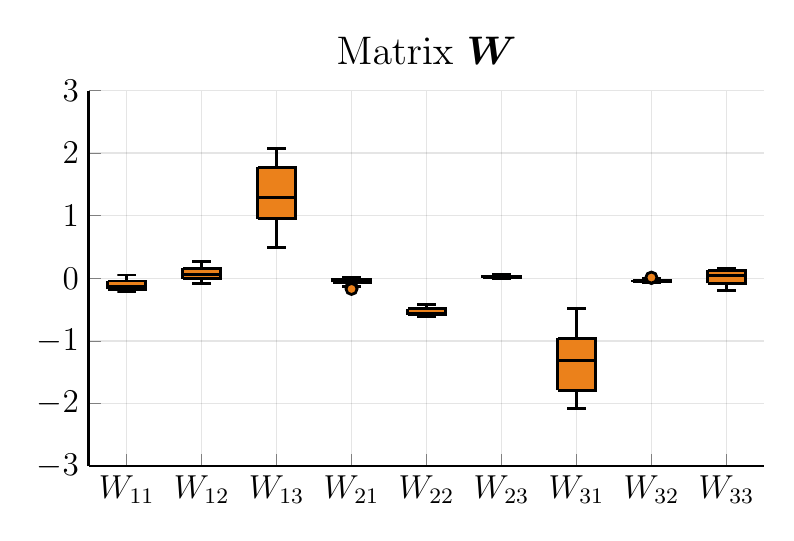
\begin{tikzpicture}[]
\begin{axis}[height = {63.5mm}, title = {Matrix $\bm W$}, xmin = {-0.0050000000000000044}, xmax = {9.005}, ymax = {3}, xlabel = {}, unbounded coords=jump,scaled x ticks = false,xlabel style = {font = {\fontsize{16 pt}{20.8 pt}\selectfont}, color = {rgb,1:red,0.00000000;green,0.00000000;blue,0.00000000}, draw opacity = 1.0, rotate = 0.0},xmajorgrids = true,xtick = {0.5,1.5,2.5,3.5,4.5,5.5,6.5,7.5,8.5},xticklabels = {$W_{11}$,$W_{12}$,$W_{13}$,$W_{21}$,$W_{22}$,$W_{23}$,$W_{31}$,$W_{32}$,$W_{33}$},xtick align = inside,xticklabel style = {font = {\fontsize{12 pt}{15.600000000000001 pt}\selectfont}, color = {rgb,1:red,0.00000000;green,0.00000000;blue,0.00000000}, draw opacity = 1.0, rotate = 0.0},x grid style = {color = {rgb,1:red,0.00000000;green,0.00000000;blue,0.00000000},
draw opacity = 0.1,
line width = 0.5,
solid},axis x line* = left,x axis line style = {color = {rgb,1:red,0.00000000;green,0.00000000;blue,0.00000000},
draw opacity = 1.0,
line width = 1,
solid},scaled y ticks = false,ylabel style = {font = {\fontsize{16 pt}{20.8 pt}\selectfont}, color = {rgb,1:red,0.00000000;green,0.00000000;blue,0.00000000}, draw opacity = 1.0, rotate = 0.0},ymajorgrids = true,ytick = {-3.0,-2.0,-1.0,0.0,1.0,2.0,3.0},yticklabels = {$-3$,$-2$,$-1$,$0$,$1$,$2$,$3$},ytick align = inside,yticklabel style = {font = {\fontsize{12 pt}{15.600000000000001 pt}\selectfont}, color = {rgb,1:red,0.00000000;green,0.00000000;blue,0.00000000}, draw opacity = 1.0, rotate = 0.0},y grid style = {color = {rgb,1:red,0.00000000;green,0.00000000;blue,0.00000000},
draw opacity = 0.1,
line width = 0.5,
solid},axis y line* = left,y axis line style = {color = {rgb,1:red,0.00000000;green,0.00000000;blue,0.00000000},
draw opacity = 1.0,
line width = 1,
solid},    xshift = 0.0mm,
    yshift = 0.0mm,
    axis background/.style={fill={rgb,1:red,1.00000000;green,1.00000000;blue,1.00000000}}
,title style = {font = {\fontsize{14 pt}{27.3 pt}\selectfont}, color = {rgb,1:red,0.00000000;green,0.00000000;blue,0.00000000}, draw opacity = 1.0, rotate = 0.0},legend style = {color = {rgb,1:red,0.00000000;green,0.00000000;blue,0.00000000},
draw opacity = 1.0,
line width = 1,
solid,fill = {rgb,1:red,1.00000000;green,1.00000000;blue,1.00000000},font = {\fontsize{12 pt}{15.600000000000001 pt}\selectfont}},colorbar style={title=}, ymin = {-3}, width = {101.6mm}]\addplot+[draw=none, color = {rgb,1:red,0.92156863;green,0.50588235;blue,0.10588235},
draw opacity = 1.0,
line width = 0,
solid,mark = *,
mark size = 2.0,
mark options = {
    color = {rgb,1:red,0.00000000;green,0.00000000;blue,0.00000000}, draw opacity = 1.0,
    fill = {rgb,1:red,0.92156863;green,0.50588235;blue,0.10588235}, fill opacity = 1.0,
    line width = 1,
    rotate = 0,
    solid
},forget plot] coordinates {
(3.5, -0.14252300560474396)
(3.5, -0.14151284098625183)
(3.5, -0.16970016062259674)
(7.5, 0.0050619496032595634)
(7.5, 0.012675742618739605)
};
\addplot+ [color = {rgb,1:red,0.00000000;green,0.00000000;blue,0.00000000},
draw opacity = 1.0,
line width = 1,
solid,mark = none,
mark size = 2.0,
mark options = {
    color = {rgb,1:red,0.00000000;green,0.00000000;blue,0.00000000}, draw opacity = 1.0,
    fill = {rgb,1:red,0.92156863;green,0.50588235;blue,0.10588235}, fill opacity = 1.0,
    line width = 1,
    rotate = 0,
    solid
},fill = {rgb,1:red,0.92156863;green,0.50588235;blue,0.10588235}, fill opacity=1.0,forget plot]coordinates {
(0.5, -0.20560422539710999)
(0.375, -0.20560422539710999)
(0.625, -0.20560422539710999)
(0.5, -0.20560422539710999)
(0.5, -0.1773149035871029)
};
\addplot+ [color = {rgb,1:red,0.00000000;green,0.00000000;blue,0.00000000},
draw opacity = 1.0,
line width = 1,
solid,mark = none,
mark size = 2.0,
mark options = {
    color = {rgb,1:red,0.00000000;green,0.00000000;blue,0.00000000}, draw opacity = 1.0,
    fill = {rgb,1:red,0.92156863;green,0.50588235;blue,0.10588235}, fill opacity = 1.0,
    line width = 1,
    rotate = 0,
    solid
},fill = {rgb,1:red,0.92156863;green,0.50588235;blue,0.10588235}, fill opacity=1.0,forget plot]coordinates {
(0.25, -0.1773149035871029)
(0.25, -0.13107550889253616)
(0.75, -0.13107550889253616)
(0.75, -0.1773149035871029)
(0.25, -0.1773149035871029)
};
\addplot+ [color = {rgb,1:red,0.00000000;green,0.00000000;blue,0.00000000},
draw opacity = 1.0,
line width = 1,
solid,mark = none,
mark size = 2.0,
mark options = {
    color = {rgb,1:red,0.00000000;green,0.00000000;blue,0.00000000}, draw opacity = 1.0,
    fill = {rgb,1:red,0.92156863;green,0.50588235;blue,0.10588235}, fill opacity = 1.0,
    line width = 1,
    rotate = 0,
    solid
},fill = {rgb,1:red,0.92156863;green,0.50588235;blue,0.10588235}, fill opacity=1.0,forget plot]coordinates {
(0.25, -0.041332364082336426)
(0.25, -0.13107550889253616)
(0.75, -0.13107550889253616)
(0.75, -0.041332364082336426)
(0.25, -0.041332364082336426)
};
\addplot+ [color = {rgb,1:red,0.00000000;green,0.00000000;blue,0.00000000},
draw opacity = 1.0,
line width = 1,
solid,mark = none,
mark size = 2.0,
mark options = {
    color = {rgb,1:red,0.00000000;green,0.00000000;blue,0.00000000}, draw opacity = 1.0,
    fill = {rgb,1:red,0.92156863;green,0.50588235;blue,0.10588235}, fill opacity = 1.0,
    line width = 1,
    rotate = 0,
    solid
},fill = {rgb,1:red,0.92156863;green,0.50588235;blue,0.10588235}, fill opacity=1.0,forget plot]coordinates {
(0.5, 0.05461854487657547)
(0.375, 0.05461854487657547)
(0.625, 0.05461854487657547)
(0.5, 0.05461854487657547)
(0.5, -0.041332364082336426)
};
\addplot+ [color = {rgb,1:red,0.00000000;green,0.00000000;blue,0.00000000},
draw opacity = 1.0,
line width = 1,
solid,mark = none,
mark size = 2.0,
mark options = {
    color = {rgb,1:red,0.00000000;green,0.00000000;blue,0.00000000}, draw opacity = 1.0,
    fill = {rgb,1:red,0.92156863;green,0.50588235;blue,0.10588235}, fill opacity = 1.0,
    line width = 1,
    rotate = 0,
    solid
},fill = {rgb,1:red,0.92156863;green,0.50588235;blue,0.10588235}, fill opacity=1.0,forget plot]coordinates {
(1.5, -0.07761125266551971)
(1.375, -0.07761125266551971)
(1.625, -0.07761125266551971)
(1.5, -0.07761125266551971)
(1.5, -0.006941249244846404)
};
\addplot+ [color = {rgb,1:red,0.00000000;green,0.00000000;blue,0.00000000},
draw opacity = 1.0,
line width = 1,
solid,mark = none,
mark size = 2.0,
mark options = {
    color = {rgb,1:red,0.00000000;green,0.00000000;blue,0.00000000}, draw opacity = 1.0,
    fill = {rgb,1:red,0.92156863;green,0.50588235;blue,0.10588235}, fill opacity = 1.0,
    line width = 1,
    rotate = 0,
    solid
},fill = {rgb,1:red,0.92156863;green,0.50588235;blue,0.10588235}, fill opacity=1.0,forget plot]coordinates {
(1.25, -0.006941249244846404)
(1.25, 0.06194778345525265)
(1.75, 0.06194778345525265)
(1.75, -0.006941249244846404)
(1.25, -0.006941249244846404)
};
\addplot+ [color = {rgb,1:red,0.00000000;green,0.00000000;blue,0.00000000},
draw opacity = 1.0,
line width = 1,
solid,mark = none,
mark size = 2.0,
mark options = {
    color = {rgb,1:red,0.00000000;green,0.00000000;blue,0.00000000}, draw opacity = 1.0,
    fill = {rgb,1:red,0.92156863;green,0.50588235;blue,0.10588235}, fill opacity = 1.0,
    line width = 1,
    rotate = 0,
    solid
},fill = {rgb,1:red,0.92156863;green,0.50588235;blue,0.10588235}, fill opacity=1.0,forget plot]coordinates {
(1.25, 0.1603672131896019)
(1.25, 0.06194778345525265)
(1.75, 0.06194778345525265)
(1.75, 0.1603672131896019)
(1.25, 0.1603672131896019)
};
\addplot+ [color = {rgb,1:red,0.00000000;green,0.00000000;blue,0.00000000},
draw opacity = 1.0,
line width = 1,
solid,mark = none,
mark size = 2.0,
mark options = {
    color = {rgb,1:red,0.00000000;green,0.00000000;blue,0.00000000}, draw opacity = 1.0,
    fill = {rgb,1:red,0.92156863;green,0.50588235;blue,0.10588235}, fill opacity = 1.0,
    line width = 1,
    rotate = 0,
    solid
},fill = {rgb,1:red,0.92156863;green,0.50588235;blue,0.10588235}, fill opacity=1.0,forget plot]coordinates {
(1.5, 0.27402302622795105)
(1.375, 0.27402302622795105)
(1.625, 0.27402302622795105)
(1.5, 0.27402302622795105)
(1.5, 0.1603672131896019)
};
\addplot+ [color = {rgb,1:red,0.00000000;green,0.00000000;blue,0.00000000},
draw opacity = 1.0,
line width = 1,
solid,mark = none,
mark size = 2.0,
mark options = {
    color = {rgb,1:red,0.00000000;green,0.00000000;blue,0.00000000}, draw opacity = 1.0,
    fill = {rgb,1:red,0.92156863;green,0.50588235;blue,0.10588235}, fill opacity = 1.0,
    line width = 1,
    rotate = 0,
    solid
},fill = {rgb,1:red,0.92156863;green,0.50588235;blue,0.10588235}, fill opacity=1.0,forget plot]coordinates {
(2.5, 0.49273577332496643)
(2.375, 0.49273577332496643)
(2.625, 0.49273577332496643)
(2.5, 0.49273577332496643)
(2.5, 0.9519701898097992)
};
\addplot+ [color = {rgb,1:red,0.00000000;green,0.00000000;blue,0.00000000},
draw opacity = 1.0,
line width = 1,
solid,mark = none,
mark size = 2.0,
mark options = {
    color = {rgb,1:red,0.00000000;green,0.00000000;blue,0.00000000}, draw opacity = 1.0,
    fill = {rgb,1:red,0.92156863;green,0.50588235;blue,0.10588235}, fill opacity = 1.0,
    line width = 1,
    rotate = 0,
    solid
},fill = {rgb,1:red,0.92156863;green,0.50588235;blue,0.10588235}, fill opacity=1.0,forget plot]coordinates {
(2.25, 0.9519701898097992)
(2.25, 1.294657289981842)
(2.75, 1.294657289981842)
(2.75, 0.9519701898097992)
(2.25, 0.9519701898097992)
};
\addplot+ [color = {rgb,1:red,0.00000000;green,0.00000000;blue,0.00000000},
draw opacity = 1.0,
line width = 1,
solid,mark = none,
mark size = 2.0,
mark options = {
    color = {rgb,1:red,0.00000000;green,0.00000000;blue,0.00000000}, draw opacity = 1.0,
    fill = {rgb,1:red,0.92156863;green,0.50588235;blue,0.10588235}, fill opacity = 1.0,
    line width = 1,
    rotate = 0,
    solid
},fill = {rgb,1:red,0.92156863;green,0.50588235;blue,0.10588235}, fill opacity=1.0,forget plot]coordinates {
(2.25, 1.771457850933075)
(2.25, 1.294657289981842)
(2.75, 1.294657289981842)
(2.75, 1.771457850933075)
(2.25, 1.771457850933075)
};
\addplot+ [color = {rgb,1:red,0.00000000;green,0.00000000;blue,0.00000000},
draw opacity = 1.0,
line width = 1,
solid,mark = none,
mark size = 2.0,
mark options = {
    color = {rgb,1:red,0.00000000;green,0.00000000;blue,0.00000000}, draw opacity = 1.0,
    fill = {rgb,1:red,0.92156863;green,0.50588235;blue,0.10588235}, fill opacity = 1.0,
    line width = 1,
    rotate = 0,
    solid
},fill = {rgb,1:red,0.92156863;green,0.50588235;blue,0.10588235}, fill opacity=1.0,forget plot]coordinates {
(2.5, 2.077324151992798)
(2.375, 2.077324151992798)
(2.625, 2.077324151992798)
(2.5, 2.077324151992798)
(2.5, 1.771457850933075)
};
\addplot+ [color = {rgb,1:red,0.00000000;green,0.00000000;blue,0.00000000},
draw opacity = 1.0,
line width = 1,
solid,mark = none,
mark size = 2.0,
mark options = {
    color = {rgb,1:red,0.00000000;green,0.00000000;blue,0.00000000}, draw opacity = 1.0,
    fill = {rgb,1:red,0.92156863;green,0.50588235;blue,0.10588235}, fill opacity = 1.0,
    line width = 1,
    rotate = 0,
    solid
},fill = {rgb,1:red,0.92156863;green,0.50588235;blue,0.10588235}, fill opacity=1.0,forget plot]coordinates {
(3.5, -0.13552163541316986)
(3.375, -0.13552163541316986)
(3.625, -0.13552163541316986)
(3.5, -0.13552163541316986)
(3.5, -0.06271143071353436)
};
\addplot+ [color = {rgb,1:red,0.00000000;green,0.00000000;blue,0.00000000},
draw opacity = 1.0,
line width = 1,
solid,mark = none,
mark size = 2.0,
mark options = {
    color = {rgb,1:red,0.00000000;green,0.00000000;blue,0.00000000}, draw opacity = 1.0,
    fill = {rgb,1:red,0.92156863;green,0.50588235;blue,0.10588235}, fill opacity = 1.0,
    line width = 1,
    rotate = 0,
    solid
},fill = {rgb,1:red,0.92156863;green,0.50588235;blue,0.10588235}, fill opacity=1.0,forget plot]coordinates {
(3.25, -0.06271143071353436)
(3.25, -0.024504529312253)
(3.75, -0.024504529312253)
(3.75, -0.06271143071353436)
(3.25, -0.06271143071353436)
};
\addplot+ [color = {rgb,1:red,0.00000000;green,0.00000000;blue,0.00000000},
draw opacity = 1.0,
line width = 1,
solid,mark = none,
mark size = 2.0,
mark options = {
    color = {rgb,1:red,0.00000000;green,0.00000000;blue,0.00000000}, draw opacity = 1.0,
    fill = {rgb,1:red,0.92156863;green,0.50588235;blue,0.10588235}, fill opacity = 1.0,
    line width = 1,
    rotate = 0,
    solid
},fill = {rgb,1:red,0.92156863;green,0.50588235;blue,0.10588235}, fill opacity=1.0,forget plot]coordinates {
(3.25, -0.011563732754439116)
(3.25, -0.024504529312253)
(3.75, -0.024504529312253)
(3.75, -0.011563732754439116)
(3.25, -0.011563732754439116)
};
\addplot+ [color = {rgb,1:red,0.00000000;green,0.00000000;blue,0.00000000},
draw opacity = 1.0,
line width = 1,
solid,mark = none,
mark size = 2.0,
mark options = {
    color = {rgb,1:red,0.00000000;green,0.00000000;blue,0.00000000}, draw opacity = 1.0,
    fill = {rgb,1:red,0.92156863;green,0.50588235;blue,0.10588235}, fill opacity = 1.0,
    line width = 1,
    rotate = 0,
    solid
},fill = {rgb,1:red,0.92156863;green,0.50588235;blue,0.10588235}, fill opacity=1.0,forget plot]coordinates {
(3.5, 0.02101919800043106)
(3.375, 0.02101919800043106)
(3.625, 0.02101919800043106)
(3.5, 0.02101919800043106)
(3.5, -0.011563732754439116)
};
\addplot+ [color = {rgb,1:red,0.00000000;green,0.00000000;blue,0.00000000},
draw opacity = 1.0,
line width = 1,
solid,mark = none,
mark size = 2.0,
mark options = {
    color = {rgb,1:red,0.00000000;green,0.00000000;blue,0.00000000}, draw opacity = 1.0,
    fill = {rgb,1:red,0.92156863;green,0.50588235;blue,0.10588235}, fill opacity = 1.0,
    line width = 1,
    rotate = 0,
    solid
},fill = {rgb,1:red,0.92156863;green,0.50588235;blue,0.10588235}, fill opacity=1.0,forget plot]coordinates {
(4.5, -0.6157950162887573)
(4.375, -0.6157950162887573)
(4.625, -0.6157950162887573)
(4.5, -0.6157950162887573)
(4.5, -0.579823449254036)
};
\addplot+ [color = {rgb,1:red,0.00000000;green,0.00000000;blue,0.00000000},
draw opacity = 1.0,
line width = 1,
solid,mark = none,
mark size = 2.0,
mark options = {
    color = {rgb,1:red,0.00000000;green,0.00000000;blue,0.00000000}, draw opacity = 1.0,
    fill = {rgb,1:red,0.92156863;green,0.50588235;blue,0.10588235}, fill opacity = 1.0,
    line width = 1,
    rotate = 0,
    solid
},fill = {rgb,1:red,0.92156863;green,0.50588235;blue,0.10588235}, fill opacity=1.0,forget plot]coordinates {
(4.25, -0.579823449254036)
(4.25, -0.5615325272083282)
(4.75, -0.5615325272083282)
(4.75, -0.579823449254036)
(4.25, -0.579823449254036)
};
\addplot+ [color = {rgb,1:red,0.00000000;green,0.00000000;blue,0.00000000},
draw opacity = 1.0,
line width = 1,
solid,mark = none,
mark size = 2.0,
mark options = {
    color = {rgb,1:red,0.00000000;green,0.00000000;blue,0.00000000}, draw opacity = 1.0,
    fill = {rgb,1:red,0.92156863;green,0.50588235;blue,0.10588235}, fill opacity = 1.0,
    line width = 1,
    rotate = 0,
    solid
},fill = {rgb,1:red,0.92156863;green,0.50588235;blue,0.10588235}, fill opacity=1.0,forget plot]coordinates {
(4.25, -0.4832053408026695)
(4.25, -0.5615325272083282)
(4.75, -0.5615325272083282)
(4.75, -0.4832053408026695)
(4.25, -0.4832053408026695)
};
\addplot+ [color = {rgb,1:red,0.00000000;green,0.00000000;blue,0.00000000},
draw opacity = 1.0,
line width = 1,
solid,mark = none,
mark size = 2.0,
mark options = {
    color = {rgb,1:red,0.00000000;green,0.00000000;blue,0.00000000}, draw opacity = 1.0,
    fill = {rgb,1:red,0.92156863;green,0.50588235;blue,0.10588235}, fill opacity = 1.0,
    line width = 1,
    rotate = 0,
    solid
},fill = {rgb,1:red,0.92156863;green,0.50588235;blue,0.10588235}, fill opacity=1.0,forget plot]coordinates {
(4.5, -0.4157397150993347)
(4.375, -0.4157397150993347)
(4.625, -0.4157397150993347)
(4.5, -0.4157397150993347)
(4.5, -0.4832053408026695)
};
\addplot+ [color = {rgb,1:red,0.00000000;green,0.00000000;blue,0.00000000},
draw opacity = 1.0,
line width = 1,
solid,mark = none,
mark size = 2.0,
mark options = {
    color = {rgb,1:red,0.00000000;green,0.00000000;blue,0.00000000}, draw opacity = 1.0,
    fill = {rgb,1:red,0.92156863;green,0.50588235;blue,0.10588235}, fill opacity = 1.0,
    line width = 1,
    rotate = 0,
    solid
},fill = {rgb,1:red,0.92156863;green,0.50588235;blue,0.10588235}, fill opacity=1.0,forget plot]coordinates {
(5.5, -0.011760009452700615)
(5.375, -0.011760009452700615)
(5.625, -0.011760009452700615)
(5.5, -0.011760009452700615)
(5.5, 0.01075523067265749)
};
\addplot+ [color = {rgb,1:red,0.00000000;green,0.00000000;blue,0.00000000},
draw opacity = 1.0,
line width = 1,
solid,mark = none,
mark size = 2.0,
mark options = {
    color = {rgb,1:red,0.00000000;green,0.00000000;blue,0.00000000}, draw opacity = 1.0,
    fill = {rgb,1:red,0.92156863;green,0.50588235;blue,0.10588235}, fill opacity = 1.0,
    line width = 1,
    rotate = 0,
    solid
},fill = {rgb,1:red,0.92156863;green,0.50588235;blue,0.10588235}, fill opacity=1.0,forget plot]coordinates {
(5.25, 0.01075523067265749)
(5.25, 0.030593860894441605)
(5.75, 0.030593860894441605)
(5.75, 0.01075523067265749)
(5.25, 0.01075523067265749)
};
\addplot+ [color = {rgb,1:red,0.00000000;green,0.00000000;blue,0.00000000},
draw opacity = 1.0,
line width = 1,
solid,mark = none,
mark size = 2.0,
mark options = {
    color = {rgb,1:red,0.00000000;green,0.00000000;blue,0.00000000}, draw opacity = 1.0,
    fill = {rgb,1:red,0.92156863;green,0.50588235;blue,0.10588235}, fill opacity = 1.0,
    line width = 1,
    rotate = 0,
    solid
},fill = {rgb,1:red,0.92156863;green,0.50588235;blue,0.10588235}, fill opacity=1.0,forget plot]coordinates {
(5.25, 0.034396715462207794)
(5.25, 0.030593860894441605)
(5.75, 0.030593860894441605)
(5.75, 0.034396715462207794)
(5.25, 0.034396715462207794)
};
\addplot+ [color = {rgb,1:red,0.00000000;green,0.00000000;blue,0.00000000},
draw opacity = 1.0,
line width = 1,
solid,mark = none,
mark size = 2.0,
mark options = {
    color = {rgb,1:red,0.00000000;green,0.00000000;blue,0.00000000}, draw opacity = 1.0,
    fill = {rgb,1:red,0.92156863;green,0.50588235;blue,0.10588235}, fill opacity = 1.0,
    line width = 1,
    rotate = 0,
    solid
},fill = {rgb,1:red,0.92156863;green,0.50588235;blue,0.10588235}, fill opacity=1.0,forget plot]coordinates {
(5.5, 0.061634622514247894)
(5.375, 0.061634622514247894)
(5.625, 0.061634622514247894)
(5.5, 0.061634622514247894)
(5.5, 0.034396715462207794)
};
\addplot+ [color = {rgb,1:red,0.00000000;green,0.00000000;blue,0.00000000},
draw opacity = 1.0,
line width = 1,
solid,mark = none,
mark size = 2.0,
mark options = {
    color = {rgb,1:red,0.00000000;green,0.00000000;blue,0.00000000}, draw opacity = 1.0,
    fill = {rgb,1:red,0.92156863;green,0.50588235;blue,0.10588235}, fill opacity = 1.0,
    line width = 1,
    rotate = 0,
    solid
},fill = {rgb,1:red,0.92156863;green,0.50588235;blue,0.10588235}, fill opacity=1.0,forget plot]coordinates {
(6.5, -2.0813913345336914)
(6.375, -2.0813913345336914)
(6.625, -2.0813913345336914)
(6.5, -2.0813913345336914)
(6.5, -1.7864260375499725)
};
\addplot+ [color = {rgb,1:red,0.00000000;green,0.00000000;blue,0.00000000},
draw opacity = 1.0,
line width = 1,
solid,mark = none,
mark size = 2.0,
mark options = {
    color = {rgb,1:red,0.00000000;green,0.00000000;blue,0.00000000}, draw opacity = 1.0,
    fill = {rgb,1:red,0.92156863;green,0.50588235;blue,0.10588235}, fill opacity = 1.0,
    line width = 1,
    rotate = 0,
    solid
},fill = {rgb,1:red,0.92156863;green,0.50588235;blue,0.10588235}, fill opacity=1.0,forget plot]coordinates {
(6.25, -1.7864260375499725)
(6.25, -1.3097766637802124)
(6.75, -1.3097766637802124)
(6.75, -1.7864260375499725)
(6.25, -1.7864260375499725)
};
\addplot+ [color = {rgb,1:red,0.00000000;green,0.00000000;blue,0.00000000},
draw opacity = 1.0,
line width = 1,
solid,mark = none,
mark size = 2.0,
mark options = {
    color = {rgb,1:red,0.00000000;green,0.00000000;blue,0.00000000}, draw opacity = 1.0,
    fill = {rgb,1:red,0.92156863;green,0.50588235;blue,0.10588235}, fill opacity = 1.0,
    line width = 1,
    rotate = 0,
    solid
},fill = {rgb,1:red,0.92156863;green,0.50588235;blue,0.10588235}, fill opacity=1.0,forget plot]coordinates {
(6.25, -0.9577610492706299)
(6.25, -1.3097766637802124)
(6.75, -1.3097766637802124)
(6.75, -0.9577610492706299)
(6.25, -0.9577610492706299)
};
\addplot+ [color = {rgb,1:red,0.00000000;green,0.00000000;blue,0.00000000},
draw opacity = 1.0,
line width = 1,
solid,mark = none,
mark size = 2.0,
mark options = {
    color = {rgb,1:red,0.00000000;green,0.00000000;blue,0.00000000}, draw opacity = 1.0,
    fill = {rgb,1:red,0.92156863;green,0.50588235;blue,0.10588235}, fill opacity = 1.0,
    line width = 1,
    rotate = 0,
    solid
},fill = {rgb,1:red,0.92156863;green,0.50588235;blue,0.10588235}, fill opacity=1.0,forget plot]coordinates {
(6.5, -0.48309987783432007)
(6.375, -0.48309987783432007)
(6.625, -0.48309987783432007)
(6.5, -0.48309987783432007)
(6.5, -0.9577610492706299)
};
\addplot+ [color = {rgb,1:red,0.00000000;green,0.00000000;blue,0.00000000},
draw opacity = 1.0,
line width = 1,
solid,mark = none,
mark size = 2.0,
mark options = {
    color = {rgb,1:red,0.00000000;green,0.00000000;blue,0.00000000}, draw opacity = 1.0,
    fill = {rgb,1:red,0.92156863;green,0.50588235;blue,0.10588235}, fill opacity = 1.0,
    line width = 1,
    rotate = 0,
    solid
},fill = {rgb,1:red,0.92156863;green,0.50588235;blue,0.10588235}, fill opacity=1.0,forget plot]coordinates {
(7.5, -0.06959563493728638)
(7.375, -0.06959563493728638)
(7.625, -0.06959563493728638)
(7.5, -0.06959563493728638)
(7.5, -0.052206890657544136)
};
\addplot+ [color = {rgb,1:red,0.00000000;green,0.00000000;blue,0.00000000},
draw opacity = 1.0,
line width = 1,
solid,mark = none,
mark size = 2.0,
mark options = {
    color = {rgb,1:red,0.00000000;green,0.00000000;blue,0.00000000}, draw opacity = 1.0,
    fill = {rgb,1:red,0.92156863;green,0.50588235;blue,0.10588235}, fill opacity = 1.0,
    line width = 1,
    rotate = 0,
    solid
},fill = {rgb,1:red,0.92156863;green,0.50588235;blue,0.10588235}, fill opacity=1.0,forget plot]coordinates {
(7.25, -0.052206890657544136)
(7.25, -0.04282580502331257)
(7.75, -0.04282580502331257)
(7.75, -0.052206890657544136)
(7.25, -0.052206890657544136)
};
\addplot+ [color = {rgb,1:red,0.00000000;green,0.00000000;blue,0.00000000},
draw opacity = 1.0,
line width = 1,
solid,mark = none,
mark size = 2.0,
mark options = {
    color = {rgb,1:red,0.00000000;green,0.00000000;blue,0.00000000}, draw opacity = 1.0,
    fill = {rgb,1:red,0.92156863;green,0.50588235;blue,0.10588235}, fill opacity = 1.0,
    line width = 1,
    rotate = 0,
    solid
},fill = {rgb,1:red,0.92156863;green,0.50588235;blue,0.10588235}, fill opacity=1.0,forget plot]coordinates {
(7.25, -0.03153342194855213)
(7.25, -0.04282580502331257)
(7.75, -0.04282580502331257)
(7.75, -0.03153342194855213)
(7.25, -0.03153342194855213)
};
\addplot+ [color = {rgb,1:red,0.00000000;green,0.00000000;blue,0.00000000},
draw opacity = 1.0,
line width = 1,
solid,mark = none,
mark size = 2.0,
mark options = {
    color = {rgb,1:red,0.00000000;green,0.00000000;blue,0.00000000}, draw opacity = 1.0,
    fill = {rgb,1:red,0.92156863;green,0.50588235;blue,0.10588235}, fill opacity = 1.0,
    line width = 1,
    rotate = 0,
    solid
},fill = {rgb,1:red,0.92156863;green,0.50588235;blue,0.10588235}, fill opacity=1.0,forget plot]coordinates {
(7.5, -0.0033302679657936096)
(7.375, -0.0033302679657936096)
(7.625, -0.0033302679657936096)
(7.5, -0.0033302679657936096)
(7.5, -0.03153342194855213)
};
\addplot+ [color = {rgb,1:red,0.00000000;green,0.00000000;blue,0.00000000},
draw opacity = 1.0,
line width = 1,
solid,mark = none,
mark size = 2.0,
mark options = {
    color = {rgb,1:red,0.00000000;green,0.00000000;blue,0.00000000}, draw opacity = 1.0,
    fill = {rgb,1:red,0.92156863;green,0.50588235;blue,0.10588235}, fill opacity = 1.0,
    line width = 1,
    rotate = 0,
    solid
},fill = {rgb,1:red,0.92156863;green,0.50588235;blue,0.10588235}, fill opacity=1.0,forget plot]coordinates {
(8.5, -0.19028207659721375)
(8.375, -0.19028207659721375)
(8.625, -0.19028207659721375)
(8.5, -0.19028207659721375)
(8.5, -0.07971572130918503)
};
\addplot+ [color = {rgb,1:red,0.00000000;green,0.00000000;blue,0.00000000},
draw opacity = 1.0,
line width = 1,
solid,mark = none,
mark size = 2.0,
mark options = {
    color = {rgb,1:red,0.00000000;green,0.00000000;blue,0.00000000}, draw opacity = 1.0,
    fill = {rgb,1:red,0.92156863;green,0.50588235;blue,0.10588235}, fill opacity = 1.0,
    line width = 1,
    rotate = 0,
    solid
},fill = {rgb,1:red,0.92156863;green,0.50588235;blue,0.10588235}, fill opacity=1.0,forget plot]coordinates {
(8.25, -0.07971572130918503)
(8.25, 0.045083945617079735)
(8.75, 0.045083945617079735)
(8.75, -0.07971572130918503)
(8.25, -0.07971572130918503)
};
\addplot+ [color = {rgb,1:red,0.00000000;green,0.00000000;blue,0.00000000},
draw opacity = 1.0,
line width = 1,
solid,mark = none,
mark size = 2.0,
mark options = {
    color = {rgb,1:red,0.00000000;green,0.00000000;blue,0.00000000}, draw opacity = 1.0,
    fill = {rgb,1:red,0.92156863;green,0.50588235;blue,0.10588235}, fill opacity = 1.0,
    line width = 1,
    rotate = 0,
    solid
},fill = {rgb,1:red,0.92156863;green,0.50588235;blue,0.10588235}, fill opacity=1.0,forget plot]coordinates {
(8.25, 0.12796640768647194)
(8.25, 0.045083945617079735)
(8.75, 0.045083945617079735)
(8.75, 0.12796640768647194)
(8.25, 0.12796640768647194)
};
\addplot+ [color = {rgb,1:red,0.00000000;green,0.00000000;blue,0.00000000},
draw opacity = 1.0,
line width = 1,
solid,mark = none,
mark size = 2.0,
mark options = {
    color = {rgb,1:red,0.00000000;green,0.00000000;blue,0.00000000}, draw opacity = 1.0,
    fill = {rgb,1:red,0.92156863;green,0.50588235;blue,0.10588235}, fill opacity = 1.0,
    line width = 1,
    rotate = 0,
    solid
},fill = {rgb,1:red,0.92156863;green,0.50588235;blue,0.10588235}, fill opacity=1.0,forget plot]coordinates {
(8.5, 0.16261924803256989)
(8.375, 0.16261924803256989)
(8.625, 0.16261924803256989)
(8.5, 0.16261924803256989)
(8.5, 0.12796640768647194)
};
\end{axis}

\end{tikzpicture}
}
      \resizebox{.075\textwidth}{.11\textwidth}{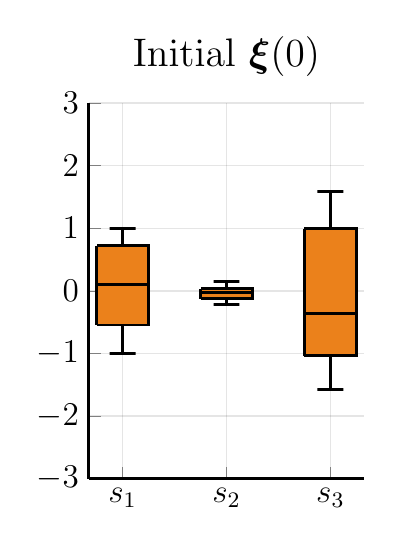
\begin{tikzpicture}[]
\begin{axis}[height = {63.5mm}, ylabel = {}, title = {Initial $\bm \xi(0)$}, xmin = {0.175}, xmax = {2.825}, ymax = {3}, xlabel = {}, unbounded coords=jump,scaled x ticks = false,xlabel style = {font = {\fontsize{16 pt}{20.8 pt}\selectfont}, color = {rgb,1:red,0.00000000;green,0.00000000;blue,0.00000000}, draw opacity = 1.0, rotate = 0.0},xmajorgrids = true,xtick = {0.5,1.5,2.5},xticklabels = {$s_1$,$s_2$,$s_3$},xtick align = inside,xticklabel style = {font = {\fontsize{12 pt}{15.600000000000001 pt}\selectfont}, color = {rgb,1:red,0.00000000;green,0.00000000;blue,0.00000000}, draw opacity = 1.0, rotate = 0.0},x grid style = {color = {rgb,1:red,0.00000000;green,0.00000000;blue,0.00000000},
draw opacity = 0.1,
line width = 0.5,
solid},axis x line* = left,x axis line style = {color = {rgb,1:red,0.00000000;green,0.00000000;blue,0.00000000},
draw opacity = 1.0,
line width = 1,
solid},scaled y ticks = false,ylabel style = {font = {\fontsize{16 pt}{20.8 pt}\selectfont}, color = {rgb,1:red,0.00000000;green,0.00000000;blue,0.00000000}, draw opacity = 1.0, rotate = 0.0},ymajorgrids = true,ytick = {-3.0,-2.0,-1.0,0.0,1.0,2.0,3.0},yticklabels = {$-3$,$-2$,$-1$,$0$,$1$,$2$,$3$},ytick align = inside,yticklabel style = {font = {\fontsize{12 pt}{15.600000000000001 pt}\selectfont}, color = {rgb,1:red,0.00000000;green,0.00000000;blue,0.00000000}, draw opacity = 1.0, rotate = 0.0},y grid style = {color = {rgb,1:red,0.00000000;green,0.00000000;blue,0.00000000},
draw opacity = 0.1,
line width = 0.5,
solid},axis y line* = left,y axis line style = {color = {rgb,1:red,0.00000000;green,0.00000000;blue,0.00000000},
draw opacity = 1.0,
line width = 1,
solid},    xshift = 0.0mm,
    yshift = 0.0mm,
    axis background/.style={fill={rgb,1:red,1.00000000;green,1.00000000;blue,1.00000000}}
,title style = {font = {\fontsize{14 pt}{27.3 pt}\selectfont}, color = {rgb,1:red,0.00000000;green,0.00000000;blue,0.00000000}, draw opacity = 1.0, rotate = 0.0},legend style = {color = {rgb,1:red,0.00000000;green,0.00000000;blue,0.00000000},
draw opacity = 1.0,
line width = 1,
solid,fill = {rgb,1:red,1.00000000;green,1.00000000;blue,1.00000000},font = {\fontsize{12 pt}{15.600000000000001 pt}\selectfont}},colorbar style={title=}, ymin = {-3}, width = {50.8mm}]\addplot+ [color = {rgb,1:red,0.00000000;green,0.00000000;blue,0.00000000},
draw opacity = 1.0,
line width = 1,
solid,mark = none,
mark size = 2.0,
mark options = {
    color = {rgb,1:red,0.00000000;green,0.00000000;blue,0.00000000}, draw opacity = 1.0,
    fill = {rgb,1:red,0.92156863;green,0.50588235;blue,0.10588235}, fill opacity = 1.0,
    line width = 1,
    rotate = 0,
    solid
},fill = {rgb,1:red,0.92156863;green,0.50588235;blue,0.10588235}, fill opacity=1.0,forget plot]coordinates {
(0.5, -1.0025405883789062)
(0.375, -1.0025405883789062)
(0.625, -1.0025405883789062)
(0.5, -1.0025405883789062)
(0.5, -0.5475115776062012)
};
\addplot+ [color = {rgb,1:red,0.00000000;green,0.00000000;blue,0.00000000},
draw opacity = 1.0,
line width = 1,
solid,mark = none,
mark size = 2.0,
mark options = {
    color = {rgb,1:red,0.00000000;green,0.00000000;blue,0.00000000}, draw opacity = 1.0,
    fill = {rgb,1:red,0.92156863;green,0.50588235;blue,0.10588235}, fill opacity = 1.0,
    line width = 1,
    rotate = 0,
    solid
},fill = {rgb,1:red,0.92156863;green,0.50588235;blue,0.10588235}, fill opacity=1.0,forget plot]coordinates {
(0.25, -0.5475115776062012)
(0.25, 0.1043335534632206)
(0.75, 0.1043335534632206)
(0.75, -0.5475115776062012)
(0.25, -0.5475115776062012)
};
\addplot+ [color = {rgb,1:red,0.00000000;green,0.00000000;blue,0.00000000},
draw opacity = 1.0,
line width = 1,
solid,mark = none,
mark size = 2.0,
mark options = {
    color = {rgb,1:red,0.00000000;green,0.00000000;blue,0.00000000}, draw opacity = 1.0,
    fill = {rgb,1:red,0.92156863;green,0.50588235;blue,0.10588235}, fill opacity = 1.0,
    line width = 1,
    rotate = 0,
    solid
},fill = {rgb,1:red,0.92156863;green,0.50588235;blue,0.10588235}, fill opacity=1.0,forget plot]coordinates {
(0.25, 0.7206912636756897)
(0.25, 0.1043335534632206)
(0.75, 0.1043335534632206)
(0.75, 0.7206912636756897)
(0.25, 0.7206912636756897)
};
\addplot+ [color = {rgb,1:red,0.00000000;green,0.00000000;blue,0.00000000},
draw opacity = 1.0,
line width = 1,
solid,mark = none,
mark size = 2.0,
mark options = {
    color = {rgb,1:red,0.00000000;green,0.00000000;blue,0.00000000}, draw opacity = 1.0,
    fill = {rgb,1:red,0.92156863;green,0.50588235;blue,0.10588235}, fill opacity = 1.0,
    line width = 1,
    rotate = 0,
    solid
},fill = {rgb,1:red,0.92156863;green,0.50588235;blue,0.10588235}, fill opacity=1.0,forget plot]coordinates {
(0.5, 0.9936660528182983)
(0.375, 0.9936660528182983)
(0.625, 0.9936660528182983)
(0.5, 0.9936660528182983)
(0.5, 0.7206912636756897)
};
\addplot+ [color = {rgb,1:red,0.00000000;green,0.00000000;blue,0.00000000},
draw opacity = 1.0,
line width = 1,
solid,mark = none,
mark size = 2.0,
mark options = {
    color = {rgb,1:red,0.00000000;green,0.00000000;blue,0.00000000}, draw opacity = 1.0,
    fill = {rgb,1:red,0.92156863;green,0.50588235;blue,0.10588235}, fill opacity = 1.0,
    line width = 1,
    rotate = 0,
    solid
},fill = {rgb,1:red,0.92156863;green,0.50588235;blue,0.10588235}, fill opacity=1.0,forget plot]coordinates {
(1.5, -0.21380501985549927)
(1.375, -0.21380501985549927)
(1.625, -0.21380501985549927)
(1.5, -0.21380501985549927)
(1.5, -0.1231940183788538)
};
\addplot+ [color = {rgb,1:red,0.00000000;green,0.00000000;blue,0.00000000},
draw opacity = 1.0,
line width = 1,
solid,mark = none,
mark size = 2.0,
mark options = {
    color = {rgb,1:red,0.00000000;green,0.00000000;blue,0.00000000}, draw opacity = 1.0,
    fill = {rgb,1:red,0.92156863;green,0.50588235;blue,0.10588235}, fill opacity = 1.0,
    line width = 1,
    rotate = 0,
    solid
},fill = {rgb,1:red,0.92156863;green,0.50588235;blue,0.10588235}, fill opacity=1.0,forget plot]coordinates {
(1.25, -0.1231940183788538)
(1.25, -0.020510799251496792)
(1.75, -0.020510799251496792)
(1.75, -0.1231940183788538)
(1.25, -0.1231940183788538)
};
\addplot+ [color = {rgb,1:red,0.00000000;green,0.00000000;blue,0.00000000},
draw opacity = 1.0,
line width = 1,
solid,mark = none,
mark size = 2.0,
mark options = {
    color = {rgb,1:red,0.00000000;green,0.00000000;blue,0.00000000}, draw opacity = 1.0,
    fill = {rgb,1:red,0.92156863;green,0.50588235;blue,0.10588235}, fill opacity = 1.0,
    line width = 1,
    rotate = 0,
    solid
},fill = {rgb,1:red,0.92156863;green,0.50588235;blue,0.10588235}, fill opacity=1.0,forget plot]coordinates {
(1.25, 0.03224852494895458)
(1.25, -0.020510799251496792)
(1.75, -0.020510799251496792)
(1.75, 0.03224852494895458)
(1.25, 0.03224852494895458)
};
\addplot+ [color = {rgb,1:red,0.00000000;green,0.00000000;blue,0.00000000},
draw opacity = 1.0,
line width = 1,
solid,mark = none,
mark size = 2.0,
mark options = {
    color = {rgb,1:red,0.00000000;green,0.00000000;blue,0.00000000}, draw opacity = 1.0,
    fill = {rgb,1:red,0.92156863;green,0.50588235;blue,0.10588235}, fill opacity = 1.0,
    line width = 1,
    rotate = 0,
    solid
},fill = {rgb,1:red,0.92156863;green,0.50588235;blue,0.10588235}, fill opacity=1.0,forget plot]coordinates {
(1.5, 0.14616471529006958)
(1.375, 0.14616471529006958)
(1.625, 0.14616471529006958)
(1.5, 0.14616471529006958)
(1.5, 0.03224852494895458)
};
\addplot+ [color = {rgb,1:red,0.00000000;green,0.00000000;blue,0.00000000},
draw opacity = 1.0,
line width = 1,
solid,mark = none,
mark size = 2.0,
mark options = {
    color = {rgb,1:red,0.00000000;green,0.00000000;blue,0.00000000}, draw opacity = 1.0,
    fill = {rgb,1:red,0.92156863;green,0.50588235;blue,0.10588235}, fill opacity = 1.0,
    line width = 1,
    rotate = 0,
    solid
},fill = {rgb,1:red,0.92156863;green,0.50588235;blue,0.10588235}, fill opacity=1.0,forget plot]coordinates {
(2.5, -1.571131706237793)
(2.375, -1.571131706237793)
(2.625, -1.571131706237793)
(2.5, -1.571131706237793)
(2.5, -1.0377112030982971)
};
\addplot+ [color = {rgb,1:red,0.00000000;green,0.00000000;blue,0.00000000},
draw opacity = 1.0,
line width = 1,
solid,mark = none,
mark size = 2.0,
mark options = {
    color = {rgb,1:red,0.00000000;green,0.00000000;blue,0.00000000}, draw opacity = 1.0,
    fill = {rgb,1:red,0.92156863;green,0.50588235;blue,0.10588235}, fill opacity = 1.0,
    line width = 1,
    rotate = 0,
    solid
},fill = {rgb,1:red,0.92156863;green,0.50588235;blue,0.10588235}, fill opacity=1.0,forget plot]coordinates {
(2.25, -1.0377112030982971)
(2.25, -0.35950733721256256)
(2.75, -0.35950733721256256)
(2.75, -1.0377112030982971)
(2.25, -1.0377112030982971)
};
\addplot+ [color = {rgb,1:red,0.00000000;green,0.00000000;blue,0.00000000},
draw opacity = 1.0,
line width = 1,
solid,mark = none,
mark size = 2.0,
mark options = {
    color = {rgb,1:red,0.00000000;green,0.00000000;blue,0.00000000}, draw opacity = 1.0,
    fill = {rgb,1:red,0.92156863;green,0.50588235;blue,0.10588235}, fill opacity = 1.0,
    line width = 1,
    rotate = 0,
    solid
},fill = {rgb,1:red,0.92156863;green,0.50588235;blue,0.10588235}, fill opacity=1.0,forget plot]coordinates {
(2.25, 0.9949156492948532)
(2.25, -0.35950733721256256)
(2.75, -0.35950733721256256)
(2.75, 0.9949156492948532)
(2.25, 0.9949156492948532)
};
\addplot+ [color = {rgb,1:red,0.00000000;green,0.00000000;blue,0.00000000},
draw opacity = 1.0,
line width = 1,
solid,mark = none,
mark size = 2.0,
mark options = {
    color = {rgb,1:red,0.00000000;green,0.00000000;blue,0.00000000}, draw opacity = 1.0,
    fill = {rgb,1:red,0.92156863;green,0.50588235;blue,0.10588235}, fill opacity = 1.0,
    line width = 1,
    rotate = 0,
    solid
},fill = {rgb,1:red,0.92156863;green,0.50588235;blue,0.10588235}, fill opacity=1.0,forget plot]coordinates {
(2.5, 1.5902372598648071)
(2.375, 1.5902372598648071)
(2.625, 1.5902372598648071)
(2.5, 1.5902372598648071)
(2.5, 0.9949156492948532)
};
\end{axis}

\end{tikzpicture}
}
      \resizebox{.075\textwidth}{.11\textwidth}{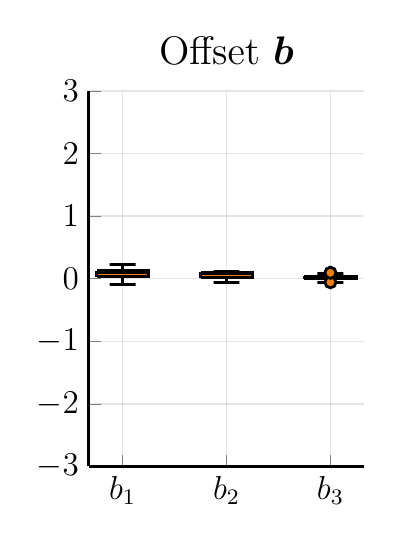
\begin{tikzpicture}[]
\begin{axis}[height = {63.5mm}, ylabel = {}, title = {Offset $\bm b$}, xmin = {0.175}, xmax = {2.825}, ymax = {3}, xlabel = {}, unbounded coords=jump,scaled x ticks = false,xlabel style = {font = {\fontsize{11 pt}{14.3 pt}\selectfont}, color = {rgb,1:red,0.00000000;green,0.00000000;blue,0.00000000}, draw opacity = 1.0, rotate = 0.0},xmajorgrids = true,xtick = {0.5,1.5,2.5},xticklabels = {$b_1$,$b_2$,$b_3$},xtick align = inside,xticklabel style = {font = {\fontsize{12 pt}{15.600000000000001 pt}\selectfont}, color = {rgb,1:red,0.00000000;green,0.00000000;blue,0.00000000}, draw opacity = 1.0, rotate = 0.0},x grid style = {color = {rgb,1:red,0.00000000;green,0.00000000;blue,0.00000000},
draw opacity = 0.1,
line width = 0.5,
solid},axis x line* = left,x axis line style = {color = {rgb,1:red,0.00000000;green,0.00000000;blue,0.00000000},
draw opacity = 1.0,
line width = 1,
solid},scaled y ticks = false,ylabel style = {font = {\fontsize{11 pt}{20.8 pt}\selectfont}, color = {rgb,1:red,0.00000000;green,0.00000000;blue,0.00000000}, draw opacity = 1.0, rotate = 0.0},ymajorgrids = true,ytick = {-3.0,-2.0,-1.0,0.0,1.0,2.0,3.0},yticklabels = {$-3$,$-2$,$-1$,$0$,$1$,$2$,$3$},ytick align = inside,yticklabel style = {font = {\fontsize{12 pt}{15.600000000000001 pt}\selectfont}, color = {rgb,1:red,0.00000000;green,0.00000000;blue,0.00000000}, draw opacity = 1.0, rotate = 0.0},y grid style = {color = {rgb,1:red,0.00000000;green,0.00000000;blue,0.00000000},
draw opacity = 0.1,
line width = 0.5,
solid},axis y line* = left,y axis line style = {color = {rgb,1:red,0.00000000;green,0.00000000;blue,0.00000000},
draw opacity = 1.0,
line width = 1,
solid},    xshift = 0.0mm,
    yshift = 0.0mm,
    axis background/.style={fill={rgb,1:red,1.00000000;green,1.00000000;blue,1.00000000}}
,title style = {font = {\fontsize{14 pt}{27.3 pt}\selectfont}, color = {rgb,1:red,0.00000000;green,0.00000000;blue,0.00000000}, draw opacity = 1.0, rotate = 0.0},legend style = {color = {rgb,1:red,0.00000000;green,0.00000000;blue,0.00000000},
draw opacity = 1.0,
line width = 1,
solid,fill = {rgb,1:red,1.00000000;green,1.00000000;blue,1.00000000},font = {\fontsize{12 pt}{15.600000000000001 pt}\selectfont}},colorbar style={title=}, ymin = {-3}, width = {50.8mm}]\addplot+[draw=none, color = {rgb,1:red,0.92156863;green,0.50588235;blue,0.10588235},
draw opacity = 1.0,
line width = 0,
solid,mark = *,
mark size = 2.0,
mark options = {
    color = {rgb,1:red,0.00000000;green,0.00000000;blue,0.00000000}, draw opacity = 1.0,
    fill = {rgb,1:red,0.92156863;green,0.50588235;blue,0.10588235}, fill opacity = 1.0,
    line width = 1,
    rotate = 0,
    solid
},forget plot] coordinates {
(2.5, 0.09276549518108368)
(2.5, -0.05793765187263489)
(2.5, 0.09336800128221512)
};
\addplot+ [color = {rgb,1:red,0.00000000;green,0.00000000;blue,0.00000000},
draw opacity = 1.0,
line width = 1,
solid,mark = none,
mark size = 2.0,
mark options = {
    color = {rgb,1:red,0.00000000;green,0.00000000;blue,0.00000000}, draw opacity = 1.0,
    fill = {rgb,1:red,0.92156863;green,0.50588235;blue,0.10588235}, fill opacity = 1.0,
    line width = 1,
    rotate = 0,
    solid
},fill = {rgb,1:red,0.92156863;green,0.50588235;blue,0.10588235}, fill opacity=1.0,forget plot]coordinates {
(0.5, -0.08775262534618378)
(0.375, -0.08775262534618378)
(0.625, -0.08775262534618378)
(0.5, -0.08775262534618378)
(0.5, 0.03313102014362812)
};
\addplot+ [color = {rgb,1:red,0.00000000;green,0.00000000;blue,0.00000000},
draw opacity = 1.0,
line width = 1,
solid,mark = none,
mark size = 2.0,
mark options = {
    color = {rgb,1:red,0.00000000;green,0.00000000;blue,0.00000000}, draw opacity = 1.0,
    fill = {rgb,1:red,0.92156863;green,0.50588235;blue,0.10588235}, fill opacity = 1.0,
    line width = 1,
    rotate = 0,
    solid
},fill = {rgb,1:red,0.92156863;green,0.50588235;blue,0.10588235}, fill opacity=1.0,forget plot]coordinates {
(0.25, 0.03313102014362812)
(0.25, 0.10017063468694687)
(0.75, 0.10017063468694687)
(0.75, 0.03313102014362812)
(0.25, 0.03313102014362812)
};
\addplot+ [color = {rgb,1:red,0.00000000;green,0.00000000;blue,0.00000000},
draw opacity = 1.0,
line width = 1,
solid,mark = none,
mark size = 2.0,
mark options = {
    color = {rgb,1:red,0.00000000;green,0.00000000;blue,0.00000000}, draw opacity = 1.0,
    fill = {rgb,1:red,0.92156863;green,0.50588235;blue,0.10588235}, fill opacity = 1.0,
    line width = 1,
    rotate = 0,
    solid
},fill = {rgb,1:red,0.92156863;green,0.50588235;blue,0.10588235}, fill opacity=1.0,forget plot]coordinates {
(0.25, 0.12942252308130264)
(0.25, 0.10017063468694687)
(0.75, 0.10017063468694687)
(0.75, 0.12942252308130264)
(0.25, 0.12942252308130264)
};
\addplot+ [color = {rgb,1:red,0.00000000;green,0.00000000;blue,0.00000000},
draw opacity = 1.0,
line width = 1,
solid,mark = none,
mark size = 2.0,
mark options = {
    color = {rgb,1:red,0.00000000;green,0.00000000;blue,0.00000000}, draw opacity = 1.0,
    fill = {rgb,1:red,0.92156863;green,0.50588235;blue,0.10588235}, fill opacity = 1.0,
    line width = 1,
    rotate = 0,
    solid
},fill = {rgb,1:red,0.92156863;green,0.50588235;blue,0.10588235}, fill opacity=1.0,forget plot]coordinates {
(0.5, 0.2208147943019867)
(0.375, 0.2208147943019867)
(0.625, 0.2208147943019867)
(0.5, 0.2208147943019867)
(0.5, 0.12942252308130264)
};
\addplot+ [color = {rgb,1:red,0.00000000;green,0.00000000;blue,0.00000000},
draw opacity = 1.0,
line width = 1,
solid,mark = none,
mark size = 2.0,
mark options = {
    color = {rgb,1:red,0.00000000;green,0.00000000;blue,0.00000000}, draw opacity = 1.0,
    fill = {rgb,1:red,0.92156863;green,0.50588235;blue,0.10588235}, fill opacity = 1.0,
    line width = 1,
    rotate = 0,
    solid
},fill = {rgb,1:red,0.92156863;green,0.50588235;blue,0.10588235}, fill opacity=1.0,forget plot]coordinates {
(1.5, -0.05768047273159027)
(1.375, -0.05768047273159027)
(1.625, -0.05768047273159027)
(1.5, -0.05768047273159027)
(1.5, 0.0182832395657897)
};
\addplot+ [color = {rgb,1:red,0.00000000;green,0.00000000;blue,0.00000000},
draw opacity = 1.0,
line width = 1,
solid,mark = none,
mark size = 2.0,
mark options = {
    color = {rgb,1:red,0.00000000;green,0.00000000;blue,0.00000000}, draw opacity = 1.0,
    fill = {rgb,1:red,0.92156863;green,0.50588235;blue,0.10588235}, fill opacity = 1.0,
    line width = 1,
    rotate = 0,
    solid
},fill = {rgb,1:red,0.92156863;green,0.50588235;blue,0.10588235}, fill opacity=1.0,forget plot]coordinates {
(1.25, 0.0182832395657897)
(1.25, 0.08106231689453125)
(1.75, 0.08106231689453125)
(1.75, 0.0182832395657897)
(1.25, 0.0182832395657897)
};
\addplot+ [color = {rgb,1:red,0.00000000;green,0.00000000;blue,0.00000000},
draw opacity = 1.0,
line width = 1,
solid,mark = none,
mark size = 2.0,
mark options = {
    color = {rgb,1:red,0.00000000;green,0.00000000;blue,0.00000000}, draw opacity = 1.0,
    fill = {rgb,1:red,0.92156863;green,0.50588235;blue,0.10588235}, fill opacity = 1.0,
    line width = 1,
    rotate = 0,
    solid
},fill = {rgb,1:red,0.92156863;green,0.50588235;blue,0.10588235}, fill opacity=1.0,forget plot]coordinates {
(1.25, 0.09744592569768429)
(1.25, 0.08106231689453125)
(1.75, 0.08106231689453125)
(1.75, 0.09744592569768429)
(1.25, 0.09744592569768429)
};
\addplot+ [color = {rgb,1:red,0.00000000;green,0.00000000;blue,0.00000000},
draw opacity = 1.0,
line width = 1,
solid,mark = none,
mark size = 2.0,
mark options = {
    color = {rgb,1:red,0.00000000;green,0.00000000;blue,0.00000000}, draw opacity = 1.0,
    fill = {rgb,1:red,0.92156863;green,0.50588235;blue,0.10588235}, fill opacity = 1.0,
    line width = 1,
    rotate = 0,
    solid
},fill = {rgb,1:red,0.92156863;green,0.50588235;blue,0.10588235}, fill opacity=1.0,forget plot]coordinates {
(1.5, 0.12207740545272827)
(1.375, 0.12207740545272827)
(1.625, 0.12207740545272827)
(1.5, 0.12207740545272827)
(1.5, 0.09744592569768429)
};
\addplot+ [color = {rgb,1:red,0.00000000;green,0.00000000;blue,0.00000000},
draw opacity = 1.0,
line width = 1,
solid,mark = none,
mark size = 2.0,
mark options = {
    color = {rgb,1:red,0.00000000;green,0.00000000;blue,0.00000000}, draw opacity = 1.0,
    fill = {rgb,1:red,0.92156863;green,0.50588235;blue,0.10588235}, fill opacity = 1.0,
    line width = 1,
    rotate = 0,
    solid
},fill = {rgb,1:red,0.92156863;green,0.50588235;blue,0.10588235}, fill opacity=1.0,forget plot]coordinates {
(2.5, -0.055338382720947266)
(2.375, -0.055338382720947266)
(2.625, -0.055338382720947266)
(2.5, -0.055338382720947266)
(2.5, -3.972277045249939e-5)
};
\addplot+ [color = {rgb,1:red,0.00000000;green,0.00000000;blue,0.00000000},
draw opacity = 1.0,
line width = 1,
solid,mark = none,
mark size = 2.0,
mark options = {
    color = {rgb,1:red,0.00000000;green,0.00000000;blue,0.00000000}, draw opacity = 1.0,
    fill = {rgb,1:red,0.92156863;green,0.50588235;blue,0.10588235}, fill opacity = 1.0,
    line width = 1,
    rotate = 0,
    solid
},fill = {rgb,1:red,0.92156863;green,0.50588235;blue,0.10588235}, fill opacity=1.0,forget plot]coordinates {
(2.25, -3.972277045249939e-5)
(2.25, 0.02092345617711544)
(2.75, 0.02092345617711544)
(2.75, -3.972277045249939e-5)
(2.25, -3.972277045249939e-5)
};
\addplot+ [color = {rgb,1:red,0.00000000;green,0.00000000;blue,0.00000000},
draw opacity = 1.0,
line width = 1,
solid,mark = none,
mark size = 2.0,
mark options = {
    color = {rgb,1:red,0.00000000;green,0.00000000;blue,0.00000000}, draw opacity = 1.0,
    fill = {rgb,1:red,0.92156863;green,0.50588235;blue,0.10588235}, fill opacity = 1.0,
    line width = 1,
    rotate = 0,
    solid
},fill = {rgb,1:red,0.92156863;green,0.50588235;blue,0.10588235}, fill opacity=1.0,forget plot]coordinates {
(2.25, 0.036873881705105305)
(2.25, 0.02092345617711544)
(2.75, 0.02092345617711544)
(2.75, 0.036873881705105305)
(2.25, 0.036873881705105305)
};
\addplot+ [color = {rgb,1:red,0.00000000;green,0.00000000;blue,0.00000000},
draw opacity = 1.0,
line width = 1,
solid,mark = none,
mark size = 2.0,
mark options = {
    color = {rgb,1:red,0.00000000;green,0.00000000;blue,0.00000000}, draw opacity = 1.0,
    fill = {rgb,1:red,0.92156863;green,0.50588235;blue,0.10588235}, fill opacity = 1.0,
    line width = 1,
    rotate = 0,
    solid
},fill = {rgb,1:red,0.92156863;green,0.50588235;blue,0.10588235}, fill opacity=1.0,forget plot]coordinates {
(2.5, 0.08242262154817581)
(2.375, 0.08242262154817581)
(2.625, 0.08242262154817581)
(2.5, 0.08242262154817581)
(2.5, 0.036873881705105305)
};
\end{axis}

\end{tikzpicture}
}
      \begin{minipage}{.28\textwidth}
        \centering
        \tikz\draw[black,fill=mLightGreen] (0,0) circle (.4ex); {\scriptsize Rodent}
      \end{minipage}
      \begin{minipage}{.28\textwidth}
        \centering
        \tikz\draw[black,fill=mLightBrown] (0,0) circle (.4ex); {\scriptsize Odent}
      \end{minipage}
    \end{tikzfigure}
    Latent codes of the Rodent compared to Odent.  All redundant parameters are
    pushed to zero by Rodent while Odent keeps one irrelevant parameter
    ($W_{22}$). Additionally we can see that the Rodent squeezes irrelevant
    parameters closer to zero than Odent.

    \vspace{1cm}
    \begin{center}
      {\huge\bf Advantages of the relevant ODE identifier}\\
    \end{center}

    \vspace{1cm}
    \begin{minipage}[t]{.28\textwidth}
    \begin{itemize}
      \item \textbf{Explainability.}  The parameters of $\bm z$ are
        decoded through an ODE solver, which gives them physical meaning.
      \item \textbf{Sparsity.} The automatic relevance determination prior on
        $\bm{z}$ encourages the simplest solution with fewest non-zero parameters.
    \end{itemize}
    \end{minipage}
    \hspace{.01\textwidth}
    \begin{minipage}[t]{.28\textwidth}
    \begin{itemize}
      \item \textbf{Partial observations.} Rodent allows learning of an ODE
        without knowledge of all state trajectories. The
        observation operator is assumed to be known.
      \item \textbf{Time series.} The convolutional part of the encoder is
        agnostic to different time series lengths.
    \end{itemize}
    \end{minipage}


  }

\block{}{
  \begin{minipage}{.05\textwidth}
    
\includegraphics[height=\textwidth]{qr-code.pdf}
  \end{minipage}
  \begin{minipage}{.37\textwidth}
    Check out the full paper at \texttt{http://tiny.cc/f6x6gz}\\
    or scan the QR code on the left! \\
    Email \texttt{niklas.heim@aic.fel.cvut.cz}
  \end{minipage}
  \begin{minipage}{.04\textwidth}
    
\includegraphics[height=\textwidth]{aic-logo.png}
  \end{minipage}
  \hspace{.03\textwidth}
  \begin{minipage}{.05\textwidth}
    
\includegraphics[height=\textwidth]{cvut-logo.jpeg}
  \end{minipage}
}

  \column{0.3}
  \block{Rodent in depth}{
    \textbf{Problem definition:} We are concerned with time series $\X = [\bm
    x_1, \bm x_2,\ldots, \bm x_K]$ with $\bm x_i \in \mathbb{R}^d$ generated
    from discrete-time, noisy observations
    \begin{equation}
      \bm x_k = H(\bm{\xi}(\Delta t k)) + e_k,
    \end{equation}
    where $k=1\ldots K$, noise $e_k \sim \N(0,\se^2\mathbf{I})$, and partial
    observation operator $H$.  The evolution of $\bm\xi(t) \in \mathbb{R}^N$ is
    governed by an ODE:
    \begin{align}
      \label{eq:dyn_sys}
      \frac{\partial \bm{\xi}}{\partial t} 
        = & f(\bm{\theta}, t) \approx \bm{W}\bm{\xi} + \bm{b}.
    \end{align}
    We aim to learn structure and order of the ODE from a set of
    trajectories $\{\X_i\}_{i=1}^{L}$  generated by the same generative process
    but with  different $\bm\theta_i$ and different $\bm\xi_i(0)$, for each
    trajectory, i.e.
    \begin{align}
      \label{eq:series_x}
      \X_i =& H(\psi(\bm\theta_i,\bm{\xi}_i(0), \bm{t}))+\bm{e},
    \end{align}
    where $\bm{t} = [0, \Delta t, \ldots, K\Delta t]$ and ODE
    solver $\psi$.  Assuming we observe a system with expected order $M$, we choose $N
    \geq M$.\\

    \textbf{Rodent:} By combining the ODE state and its parameters in
    $\z=[\bm\theta,\bm\xi(0)]$ we can define the data likelihood as
    \begin{align}
      \label{eq:decoder}
      p(\x|\z) &= \N(\x|H(\psi(\z)),\sigma_x^2).
    \end{align}
    To determine the structure of the ODE, we employ the ARD prior:
    \begin{align}
      \label{eq:ard_model}
      p(\z) &= \N(\z|0,\text{diag}(\laz^2)) &
      p(\laz) &= 1/\laz.%\Gamma(\laz|\alpha_0, \beta_0)
    \end{align}

    The posterior of $\bm z$ is prescribed by
    \begin{align}
      \label{eq:ard_posterior}
      p(\z|\x) = \N(\z|\phi_\omega(\x), \bm{\sigma}_z^2)
    \end{align}
    where mean $\mz=\phi_\omega(\x)$ is a neural net with parameters
    $\omega$.
    The resulting ELBO:
    {\fontsize{25}{20}
    \begin{equation}
    \begin{aligned}
      \label{eq:elbo_reparam}
      \mathcal{L} &= \sum_{i=1}^n \E{p(z|x)}{\frac{(\x_i - \psi(\phi_\omega(\x_i) + \bm{\sigma}_z \odot \bm{\epsilon}))^2}{2\se^2}}
                  + \frac{nd}{2}\log(\se) \\
                  &+ \sum_{i=1}^n \left(
                      \log\left(\frac{\laz^2}{\sz^2}\right)
                      -m + \frac{\sz^2}{\laz^2} + \frac{\phi_\omega(\x_i)^2}{\laz^2}
                  \right),
    \end{aligned}
    \end{equation}}
    with Gaussian noise $\bm{\epsilon} \sim \N(0,I)$, decoder
    $H(\psi(\bm\theta,\bm\xi(0)))\equiv\phi(\z)$, and $\text{dim}(\z) = m$.\\

    \textbf{Encoder:} The encoder $\phi_\omega$ consists of two parts: (i) A
    dense net that receives only a few steps of the beginning of the time
    series, responsible for predicting $\bm \xi(0)$. (ii) A CNN that predicts
    $\bm \theta$.  The CNN averages over the time dimension after the
    convolutions, which makes it possible to use samples of different length.\\

    \textbf{Reidentification:} We sample a batch of
    latent codes from the encoder for each input.  The samples
    are used as starting points for another optimization of the reconstruction
    error $R$
    \begin{equation}
      R = \mathrm{MSE}(\phi(\bm z) - \x),
    \end{equation}
    while keeping all irrelevant parameters fixed.
    On the left, four parameters, namely $W_{13}$,
    $W_{31}$, $\xi_{1}$, and $\xi_{3}$ were found to be relevant, so only
    those are changing during the optimization with respect to $R$.
    This means that we stay in the identified model manifold, but are able to
    extrapolate far beyond the training range.   

    \vspace{5.20cm}
  }
  
\end{columns}

\end{document}
